%%%%%%%%%%%%%%%%%%%%%%%%%%%%%%%%%%%%%%%%%%%%%%%%%%%%%%%%%%%%%
% Matt Pitkin 26/04/05                                      %
%                                                           %
% Chapter 2: Neutrons stars and other such stuff ...        %
%%%%%%%%%%%%%%%%%%%%%%%%%%%%%%%%%%%%%%%%%%%%%%%%%%%%%%%%%%%%%

\chapquote{I hate to go all technical on you, but... all hands on deck, swirly thing alert!}{Cat -
Red Dwarf}

%\chapter{Neutrons stars and other such stuff}
\chapter{Gravitational waves from known pulsars}
% quick description of chapter contents
In this chapter we will discuss pulsars as a source of continuous gravitational waves. A search
technique and parameter estimation tool for such sources is described. The inclusion of timing
noise corrections and binary pulsar time delays into this search is then discussed, along with code
validation proceedures.

% first section will review pulsars and possible gravitational wave emission mechanisms
% will introduce gws from glitches in chapter 4
\section{Pulsars and gravitational radiation}
One class of astrophysical object thought to be a strong candidate for the emission of detectable
continuous \gws is neutron stars. These are the ultra-dense evolutionary end states for high mass
stars ($\sim 8-25\,M_\odot$) produced during core-collapse in a Type II supernova, or accretion
induced collapse of a white dwarf in a Type I supernova. They were theorised (in the first instance
by Baade and Zwicky, 1934 \cite{Baade:1934}) for several decades before evidence for their existence
was confirmed by the discovery of pulsars in 1967 by Hewish and Bell \cite{HewishBell:1968}. They
discovered periodic coherent radio pulses from outside the solar system. These were consistent with
a beamed source of radiation from a rapidly rotating highly magnetic object. The very fast periods
seen for the promptly discovered Crab and Vela pulsars ruled out, as sources, already known objects
such a white dwarfs as they would have radii greater than the surface of the light
cylinder\footnote{The surface which would be rotating at the speed of light.}. This left the far
denser and smaller neutron stars as the prime candidate. The pulsed emission was due to an offset
between the spin axis and magnetic axis, from which electromagnetic radiation was being beamed,
occurring when the magnetic axis crossed our line of sight; in a way analogous to a lighthouse.
Since their initial discovery, at the time of writing, 1533 pulsars have been discovered (as given
by the Australia Telescope National Facility - ATNF - online pulsar catalogue \cite{ATNF}). The
majority have been discovered through radio surveys of the sky, although emission from some objects
can be seen across a wide range of energies, even into the $\gamma$-ray spectrum. Surveys are
ongoing, but estimates of the number of pulsars in the galaxy can be made by inference from the
current population, taking into account biasing from selection effects, and the supernova rate.
Estimates give values of $\sim 200\,000$ active pulsars within our galaxy (see Lorimer, 2001
\cite{Lorimer:2001}).

Pulsars are found in a wide range of environments. As might be expected from their birth in
supernovae some are found associated with supernova remnants (SNR). These are typically young
pulsars whose birth velocity has not yet caused a large displacement from the remnant, their
emissions are still enough to excite the SNR to emit, and the SNR has not dissipated into the
interstellar medium (ISM). Other pulsars are found in binary systems as companions to a whole range
of bodies ranging from planets, through main sequence stars, to white dwarfs and other neutron
stars. The so called millisecond pulsars (pulsars with rotation periods of $< 10$ milliseconds) are
often found within binary systems, and their rotation speed is often attributed to their being
spun-up by accretion of material from a stellar companion. Many pulsars are seen within globular
clusters, which is not surprising due to the high concentration of old stars. Pulsars are also seen
without any association. From here on we shall classify any pulsar not in a binary system as
isolated. 

The range of spin periods covered by pulsars is quite wide going from $\sim 12$ seconds to
$\sim 1.5$ milliseconds. The distribution of periods is not uniform with distinct populations of
fast millisecond and young pulsars, and slower pulsars. 

Pulsars are generally seen to spin-down as they lose rotational energy via various emission
mechanisms. The generally accepted energy loss is via magnetic dipole radiation. The energy loss
mechanism most important for us would be via gravitational radiation. The phase evolution of a
pulsar can generally be well described by the Taylor expansion,
\begin{equation}\label{PhaseTaylorExp}
\phi(t) = \phi_0 + 2\pi{}\left\{\nu_0(t-t_0) + \frac{1}{2}\dot{\nu_0}(t-t_0)^2 +
\frac{1}{6}\ddot{\nu_0}(t-t_0)^3 + \ldots\right\},
\end{equation}
where $\phi_0$ is the initial phase, $\nu_0$ and its time derivatives are the pulsar frequency and
spin-down coefficients at an epoch $t_0$, and $t$ is the time in a reference frame comoving with the
pulsar. For the vast majority of pulsars the value of $\dot{\nu}$ is very small and $\ddot{\nu}$ is
unmeasurable or swamped by timing noise (see \S\ref{TimingNoise}). To date there are only five
pulsars with well enough sampled observations to have a measurable $\ddot{\nu}$, which allows a
quantity called the braking index, $n = \frac{\nu\ddot{\nu}}{\dot{\nu}^2}$, to be defined. For spin
down caused by pure magnetic dipole radiation then $n=3$, and for pure gravitational radiation $n=5$
(see Palomba, 2000 \cite{Palomba:2000}). For the few pulsars with a measurable value of the breaking
index, four (PSR\,J0534+2200 - the Crab pulsar, PSR\,J1513-5908, PSR\,J0835-4510 - the Vela
pulsar, and PSR\,J0540-6919) show $n<3$ \cite{Palomba:2000} and one (PSR\,J0537-6910) shows $n \sim
6.9$ \cite{Marshall:2004}. For the four pulsars with $n<3$ Palomba \cite{Palomba:2000} tries to
explain them with a combination of magnetic breaking and gravitational radiation. 

Neutron stars are typically thought, from theoretical arguments, to have a mass of around
1.4\,${\rm M}_\odot$ and radii of $\sim 10$\,km. Using these canonical values of mass and radius and
assuming a uniform density sphere, the moment of inertia of a neutron star is often quoted as $I =
\frac{2}{5}MR^2 = 10^{38}\rm{kg}\,\rm{m}^2$. Their structure is thought to consist of a thin crust
of highly distorted heavy nuclei (mostly iron) and a degenerate electron gas, above a mantle of
fluid neutrons with some protons and electrons, surrounding a core of neutrons or unbound quarks
(this is discussed in more detail in Benhar, 2005 \cite{Benhar:2005}). Densities range from $\sim
10^{10}$\,kg/${\rm{m}}^3$ near the surface to $\sim 10^{18}$\,kg/${\rm{m}}^3$ in the core. The true
nature of the neutron star interior is unknown, with much speculation surrounding the possibility of
it consisting of strange quark matter and other exotic theories. Questions about the
equation-of-state could possibly be answered through observations of \gws from neutron stars. 

\subsection{Gravitational wave emission mechanisms}
Spinning stars with perfect symmetry about their rotation axis will not emit gravitational waves, so
if we expect to detect any continuous \gw signal then some mechanism must be in place to cause an
asymmetry to arise. In this section the most important \gw emission mechanism we will discuss is the
emission of continuous waves from a triaxial neutron star (in Chapter 4 the emission of transient
quasi-normal modes will be discussed).

\subsubsection{Emission from a triaxial neutron star}
There are several ways in which a neutron star could be deformed from asymmetry. During formation
and crystallisation the neutron star crust may be deformed from axisymmetry due to centrifugal
forces. This deformation could then be supported by the solid crust \cite{Pandharipande:1976}.
Another possibility is that a strong magnetic field could distort the star. Gravitational waves
produced by such mechanisms would be produced at twice the rotation frequency of the star. They
would have a characteristic strain amplitude given by
\begin{equation}\label{Pulsarh0}
h_0 = \frac{16\pi^2G}{c^4}\frac{\varepsilon I_{zz}\nu^2}{r},
\end{equation}
where $\nu$ is the star's spin frequency, $I_{zz}$ is the principal moment of inertia, $\varepsilon$
is the star's ellipticity, and $r$ is the distance to the star (see Jaranowski {\it et al.}, 1998
\cite{JKS:1998}). In this chapter and the next we shall only consider \gws emitted via this
mechanism.

\subsubsection{Emission from a precessing neutron star}
Precession of a star about its rotation axis is another source of asymmetry. Gravitational waves
generated by precession would have a frequency at the star's rotation frequency, with sidebands
ofset by the precession frequency from this for small wobble angles (Zimmermann and Szedentis, 1979
\cite{Zimmermann:1979}). In Jones and Andersson (2002) \cite{JonesAndersson:2002} they conclude that
gravitational wave amplitudes from such sources are likely to be orders of magnitude below the level
of detectability for LIGO, but may be detectable with AdvLIGO.

\subsubsection{Other mechanisms}
Another source of asymmetry in a star may arise if it is in a binary system and accreting matter
from its companion, as in Low Mass X-ray Binaries (LMXBs). Such systems could emit gravitational
waves via $r$-modes as discussed in Andersson {\it et al.} (1999) \cite{Andersson:1999} or could
perhaps have large ellipticities induced by an accretion-confined magnetic field as in Melatos and
Payne (2005) \cite{MelatosPayne:2005}.

\subsection{Gravitational wave searches}
Known pulsars provide an enticing target for \gw searches. With known positions and frequencies the
parameter space to search over can be much smaller than for unknown searches. The fact that the
waves are continuous means that, assuming a coherent search, you can build up signal-to-noise with
longer observations (scaling as $\sqrt{T}$, where $T$ is observation time). The main drawback in
a search for \gws for the majority of known pulsars is that the level of emission can be inferred
to be much lower than current detector sensitivities. It is possible using existing radio
measurement to set an upper limit on \gw emission amplitudes from energy conservation arguments,
assuming there is no unknown mechanism powering the star in some way. If one assumes that
all the kinetic energy lost as the pulsar spins-down is dissipated via gravitational radiation
(${\rm{d}}E_{\rm{gw}}/{\rm{d}}t = 4\pi^2I_{zz}\nu|\dot{\nu}|$) then an upper limit on $h_0$ can be
set as
\begin{equation}\label{spindownUL}
h_0^{\rm{spin-down}} = \left(\frac{5}{2}\frac{GI_{zz}\dot{\nu}}{c^3r^2\nu}\right)^{1/2},
\end{equation}
this will be discussed in more detail in \S\ref{astrophysics}. Even so, searches do provide upper
limits on emission which can be valuable in constraining certain equations of state, and we may just
find something!
 
The ability to search for \gws from known pulsars before the advent of the large scale
interferometric detectors was rather limited. Bar detectors are only sensitive in a narrow band of
frequencies around their resonant frequencies and so cannot be used to target objects outside
that band. A specific attempt to search for \gws from the Crab pulsar at a frequency of
$\sim 60.2$\,Hz\footnote{twice its rotation frequency at the time of their search, although the
frequency now searched is closer to $\sim 59.6$\,Hz.}, was made with a specially designed aluminium
quadrupole antenna (see Hirakawa {\it et al.}, 1978 and Suzuki, 1995 \cite{Hirakawa:1978,
Suzuki:1995}). A search for \gws from the then fastest millisecond pulsar, PSR\,J1939+2134, was
conducted by Hough {\it et al} (1983) \cite{Hough:1983} using a split bar detector, producing an
upper limit of $h_0 < 10^{-20}$. 

Using the inherently broadband interferometers a larger sample of objects is accessible. The first
search for \gws from a pulsar using an interferometer was with the prototype 40\,m interferometer at
Caltech by Hereld (1983) \cite{Hereld:1983}. Again the search was for \gws from PSR\,J1939+2134, and
produced upper limits of $h_0 < 3.1\ee{-17}$ and $h_0 < 1.5\ee{-17}$ for the first and second
harmonics of the pulsar's rotation frequency. For the LIGO instruments all pulsars with rotation
frequencies $> 25$\,Hz (\gw frequency $> 50$\,Hz) are accessible. Below this frequency the seismic
noise floor rises sharply giving far less stationary data and sensitivities well below sensible
levels. This generally leaves only the population of millisecond and young pulsars accessible,
consisting of 150 pulsars at the time of writing (from the ATNF catalogue \cite{ATNF}). The  low
frequency sensitivity of the VIRGO detector may in the future allow the probing of a larger sample
of pulsars at lower frequencies.

\subsubsection{Current searches}
The search for \gws from known pulsars has developed rapidly since the start of data taking runs
with the LIGO and \geo interferometers in 2002. Data from the first science run (S1) was used to
perform a search for \gws from PSR\,J1939+2134, assuming a triaxial star emitting at twice the
rotation frequency \cite{Abbott:2004}. For this search two techniques were used: one a frequency
domain, frequentist search, and the other a time domain, Bayesian search. 

\subsubsection{The frequency domain method and others}
The frequency domain search makes use of Fourier transforms of the data to search for a signal in
the correct frequency bin using a detection statistic ($\mathcal{F}$-statistic \cite{JKS:1998}).
This statistic is based on a maximum-likelihood analysis, making use of the output of
matched-filters (more on matched filtering is given in \S\ref{matchedfiltering}) for a series of
templates over the pulsar signal parameters. An upper limit using this statistic can be set
using Monte-Carlo injections and establishing a threshold which gives a certain false alarm rate and
false dismissal rate.

There are efforts to search for \gws from neutron stars by a variety of other methods in the LSC
using LIGO and \geo data from the last four science runs. The use of the Hough transform method can
be seen in Abbott {\it et al.} (2005c) \cite{Abbott3:2005}, the StackSlide method is described in
Mendell (2005) \cite{Mendell:2005}, and the PowerFlux method is described in Dergachev (2005)
\cite{Dergachev:2005}. These generally make use of short Fourier transformed stretches of data to
form something analogous to a time-frequency spectrogram. Techniques are used to modulate this in a
way consistent with the expected \gw form. The spectrogram is then searched for evidence of a signal
using a variety of pattern recognition procedures.

These methods do not rely on precise knowledge of the signal phase evolution like the time
domain method. This lends them to uses in all-sky searches over large frequency and spin-down ranges
rather than being used to target specific objects. They can also be used in targeted searches for
objects with badly constrained parameters, for example the search for \gws from the LMXB systems.
These strategies can also be used in hierarchical searches as described in Brady and Creighton
(2000) \cite{BradyCreighton:2000}, whereby wide area searches provide possible signal candidates for
a more tightly focused follow up search. Coincidences between candidates in different detectors can
also be applied.

For the analysis of the second science run (S2) of the LIGO interferometers the first attempt to
search for a broad range of pulsars was made. Twenty eight pulsars with either very well defined and
stable parameters or with new timing taken over the period of S2 were searched for
\cite{Abbott:2005}. All these pulsars were isolated. For this search a slightly modified version of
the time domain method of S1 was used. It is this search method which will be discussed in more
detail below and which has been used to obtain the results herein.

Another method making use of the time domain technique and Markov Chain Monte Carlo (MCMC)
statistical methods is also being explored for possible ``fuzzy'' targeted searches where some
signal parameters are badly constrained (see Veitch {\it et al.}, 2005 \cite{Veitch:2005}). An MCMC
approach provides a way of intelligently exploring large parameter spaces without having to
exhaustively cover the entire range. An example of an object for which such a search is being
applied is a potential pulsar remnant of SN1987A (a supernova which occurred in the LMC in 1987), as
speculatively observed by Middleditch {\it et al.} (2000) \cite{Middleditch:2000}, where the pulsar
frequency and spin-down are uncertain within a small range. Problems with this technique are that it
does not naturally lend itself to producing an upper limit (rather than a detection), although
further study is going into this area.

% second section will review the time domain search method for gravitational waves from known
% pulsars - may have a short review of other searches (or leave in introduction
\section{Time domain search method}\label{TimeDomainMethod}
The time domain method described here is described more fully in Dupuis (2004) and Dupuis and Woan
(2005) \cite{Dupuis:2004, DupuisWoan:2005}. The extensions to this included here are the additions
of timing noise corrections and binary system effects into the model. We receive data from the \gw
sensitive channels of the LIGO and \geo interferometers. For LIGO data this is received in an
uncalibrated form (raw voltages from the instrument output) with frequency domain calibration
information supplied separately (calibration will be discussed in more detail in Chapter 3). For
\geo time series data is supplied in a calibrated form, making post-processing calibration
unnecessary. All data is received at a sampling rate of 16\,384\,Hz. This sampling rate means a
frequency range of 8192\,Hz is available for searches. In known pulsar searches the frequency is
known very precisely, so the vast majority of this frequency space is redundant. A way to
down-sample this large bandwidth of data is useful to increase the speed of any search. Knowledge of
the pulsar parameters allows us to perform a heterodyne on the data and down-sample it to
$\frac{1}{60}$\,Hz (one sample per minute), as described later.

The expected signal from a pulsar is given by
\begin{equation}\label{PulsarSignal}
h(t) = \frac{1}{2}F_+(t;\psi)h_0(1+\cos^2\iota)\cos{2\phi(t)} +
F_{\times}(t;\psi)h_0\cos{\iota}\sin{2\phi(t)},
\end{equation}
where $\phi(t)$ is that given in equation~\ref{PhaseTaylorExp}, $F_+$ and $F_{\times}$ are the
detector beam patterns for the plus and cross polarisations of the gravitational waves, $\psi$ is
the wave polarisation angle, and $\iota$ is the angle between the rotation axis of the pulsar and
the line-of-sight. For a gravitational wave signal impinging on the Earth the signal arrival time at
the detector, $t$, given in equation~\ref{PhaseTaylorExp} will be modulated by Doppler, time delay
and relativistic effects caused by the motions of the Earth and other bodies in the solar system.
Therefore,
\begin{equation}\label{TimeDelay}
t_b = t + \delta{}t = t + \frac{\mathbf{r}\cdot\hat{\mathbf{n}}}{c} + \Delta_{E_{\odot}} +
\Delta_{S_{\odot}}, 
\end{equation}
where $\mathbf{r}$ is the position of the detector with respect to the solar system barycentre
(SSB), $\hat{\mathbf{n}}$ is the unit vector pointing to the pulsar, $\Delta_{E_{\odot}}$ is the
special relativistic Einstein delay, and $\Delta_{S_{\odot}}$ is the general relativistic Shapiro
delay. This corrects the signal to the SSB time $t_b$. This reference frame is assumed to be at
rest with respect to the pulsar, with its proper motion generally being negligible. For pulsar's in
binary systems there will be additional time delays as discussed in \S\ref{Binaries}.

We assume that our \gw detector data is given by
\begin{equation}
s(t) = h(t) + n(t),
\end{equation}
where $h(t)$ is the \gw signal and $n(t)$ is the noise. In searching for a particular pulsar we can
perform a complex heterodyne of the data by multiplying it by $e^{-i2\phi(t_b)}$, where $\phi(t_b)$
is the phase evolution of that pulsar given by equation~\ref{PhaseTaylorExp}, and $t_b$ from
equation~\ref{TimeDelay}. The pulsar signal (equation~\ref{PulsarSignal}) can be rewritten using
trigonometric identities as
\begin{equation}
h(t) = A_1(t)e^{i2\phi(t_b)} + A_2(t)e^{-i2\phi(t_b)},
\end{equation}
where
\begin{equation}
A_1(t) = \frac{1}{4}F_{+}(t;\psi)h_0(1+\cos^2\iota)e^{i2\phi_0} -
\frac{i}{2}F_{\times}(t;\psi)h_0\cos{\iota}e^{i2\phi_0},
\end{equation}
and
\begin{equation}
A_2(t) = \frac{1}{4}F_+(t;\psi)h_0(1+\cos^2\iota)e^{-i2\phi_0} +
\frac{i}{2}F_{\times}(t;\psi)h_0\cos{\iota}e^{-i2\phi_0},
\end{equation}
and $\phi_0$ is the initial phase of the \gw signal from the pulsar. Performing the heterodyne on
the signal transforms
\begin{equation}
s(t) \to s(t)e^{-i2\phi_0} = s_{\rm{het}}(t) = (h(t)+n(t))e^{-i2\phi_0} = A_1(t) +
A_2(t)e^{-i4\phi(t_b)} + n(t)e^{-i2\phi(t_b)}
\end{equation}
which removes the phase evolution from the $A_1$ term and increases the oscillation of the $A_2$
term to twice the \gw frequency. $A_1(t)$ will now only oscillate at the diurnal rate of the
detector antenna pattern. The slow rate of change of the antenna pattern means that the data can be
significantly down-sampled by averaging from 16\,384\,Hz to $\frac{1}{60}$\,Hz. We call each
minute sample $B_k$ where $k$ is the sample number. Before this averaging takes place it is prudent
to low-pass filter the data to prevent aliasing from other bands contaminating the pulsar signal
band. The filters used are three consecutive third order Butterworth infinite impulse response (IIR)
filters, with a cut-off frequency of $\frac{1}{2}$\,Hz. This should also effectively suppress the
fast oscillating $A_2(t)$ term. After filtering, the data can then be averaged to give
\begin{equation}
B_k = \frac{1}{M}\sum_{i=1}^M s'_{\rm{het}}(t_i),
\end{equation}
where $s'_{\rm{het}}$ is the filtered heterodyned data and $M=16\,384\,{\rm Hz}\times60\,{\rm s} =
983\,040$. The averaging will also act as another level of low pass filtering. In this approach the
pulsar phase and therefore solar system barycentring time delays need to be calculated for every
sample of data at 16\,384\,Hz. This can be computationally expensive, but does mean that the filter
cut-off frequencies can be tight and the data averaged to a low rate. If the pulsar parameters were
not well known, so that the signal could drift across the heterodyned band, then the filter cut-offs
and re-sampling rate might need to be increased. This can be done on purpose to try to reduce the
computation time. For example an initial heterodyne using a phase calculated with just the pulsar
frequency and without the barycentring can be carried out. The data can then be re-sampled to, say,
4\,Hz and re-heterodyned with the frequency derivatives and barycentre timing corrections included.
When performing such an analysis for a few pulsars the former strategies' computational time is not
too constraining, but for many pulsars it can become quite inefficient. 

\subsection{Bayesian analysis}
Once the data has been heterodyned we are left with the complex value
\begin{equation}\label{Bofk}
B_k = \frac{1}{4}F_+(t_k;\psi)h_0(1+\cos^2\iota)e^{i2\phi_0} -
\frac{i}{2}F_{\times}(t_k;\psi)h_0\cos{\iota}e^{i2\phi_0}+n(t_k)',
\end{equation}
where $n(t_k)'$ is the heterodyned averaged noise for the $k^{\rm{th}}$ sample. We want to
somehow search for the signal buried in this noise. This signal is defined by the four unknown
parameters of $h_0$, $\psi$, $\iota$ and $\phi_0$.

To search for the signal we use a Bayesian parameter estimation method. Two slightly different
approaches to this are considered in Dupuis (2004) \cite{Dupuis:2004}, one in which the noise
variance is estimated from the data and one in which the noise variance is considered to be unknown.
Here we will concentrate on the latter method. Bayesian statistics make use of the basic rules of
probability theory, namely the product rule and the sum rule. Application of these leads to Bayes'
theorem,
\begin{equation}\label{Bayes}
p(x|y,I) = \frac{p(y|x,I)\times{}p(x|I)}{p(y|I)},
\end{equation}
where $p(x|y,I)$ is called the posterior probability distribution function (pdf) of $x$ given $y$,
$p(y|x,I)$ is the likelihood function of $y$ given $x$, $p(x|I)$ is the prior probability
distribution of $x$.

In our search we start off with the Gaussian likelihood function as representing the likelihood of
each complex $B_k$,
\begin{equation}
p(B_k| \mathbf{a},\sigma_k) = \frac{1}{(\sigma_k\sqrt{2\pi})^2}\exp\left(-\frac{| B_k -
y_k |^2}{2\sigma_k^2}\right),
\end{equation} 
where $\mathbf{a} = \{h_0, \psi, \iota, \phi_0\}$, $y_k = B_k - n(t_k)'$ is our model, and
$\sigma_k$ is the standard deviation of the noise in $B_k$. It is shown in Bretthorst (1988)
\cite{Bretthorst:1988} that such a likelihood function is the least informative. This is not to say
that it is a bad likelihood function to use, but just means that it is expressing the least prior
information on what the distribution looks like. If we assume that the noise in each $B_k$ is
independent then our complete likelihood for the whole set of data can be given by the product of
all the Gaussians,
\begin{equation}\label{GaussianLikelihood}
%p(\{B_k\}| \mathbf{a},\{\sigma_k\})=\frac{1}{(\sigma_k\sqrt{2\pi})^{2n}}\exp\left(-\sum_{k=1}
%^n\frac{| B_k - y_k |^2}{2\sigma_k^2}\right), 
p(\{B_k\}| \mathbf{a},\{\sigma_k\})=
\left(\prod_{k=1}^n\frac{1}{(\sigma_k\sqrt{2\pi})^2}\right)\exp\left(-\sum_{k=1}^n\frac{| B_k - y_k
|^2}{2\sigma_k^2}\right),
\end{equation}
where $n$ is the number of $B_k$s. In the search of Abbott {\it et al.} (2004a) \cite{Abbott:2004}
this likelihood was used with the standard deviation of each $B_k$ calculated before the
down-sampling took place. In a strict sense the Gaussian likelihood should only be used when the
noise level is known in advance, whereas in \cite{Abbott:2004} it was estimated from the data. This
can lead to non-negligible uncertainties in $\sigma$ when the number of data points used to estimate
it is low. In subsequent searches \cite{Abbott:2005, Dupuis:2004} the above likelihood was adapted
for the case where the noise variance was unknown. This is achieved by taking the variance as an
unknown nuisance parameter and marginalising over it for segments of data when the noise level can
be assumed to be stationary. If we split the $n$ $B_k$s into $M$ segments of length $m_j$ with the
same noise level then
\begin{equation}
n = \sum_{j=1}^M m_j.
\end{equation}
The likelihood for each segment $j$ can be rewritten as
\begin{eqnarray}\label{MarginaliseNoiseLikelihood}
p(\{B_k\}_j|\mathbf{a}) & \propto & \int_0^\infty p(\{B_k\}_j,\sigma_j|\mathbf{a})\rm{d}\sigma_j
\nonumber \\
 & \propto & \int_0^\infty p(\sigma_j|\mathbf{a})p(\{B_k\}_j|\mathbf{a},\sigma_j)\rm{d}\sigma_j,
\end{eqnarray}
where $p(\sigma_j|\mathbf{a})$ is the prior on the noise floor and the likelihood is the Gaussian
likelihood given in equation~\ref{GaussianLikelihood}. As $\sigma_j$ is a scale parameter the least
informative prior on it is the Jeffreys' prior (uniform in log space)
\begin{eqnarray}\label{NoisePrior}
p(\sigma_j|\mathbf{a}) & \propto \frac{1}{\sigma_j} & (\sigma_j \ge 0), \\
 & =0 & (\sigma_j < 0). \nonumber
\end{eqnarray}
Combining the prior in equation~\ref{NoisePrior} with equation~\ref{MarginaliseNoiseLikelihood}
gives a likelihood integral
\begin{equation}\label{NoiseIntegral}
p(\{B_k\}_j|\mathbf{a}) \propto \int_0^\infty
\frac{1}{\sigma_j^{2m_j+1}}\exp\left(-\frac{1}{2\sigma_j^2}\sum_{k=1}^{m_j}|B_k - y_k|^2\right)
\rm{d}\sigma_j.
\end{equation}
This integral can be solved analytically following the procedure given in \cite{Dupuis:2004}.
Making the substitutions
\begin{eqnarray}
u^2 & = & \frac{\sum{}|B_k-y_k|^2}{2\sigma_j^2}, \\
\rm{d}u & = & -\frac{\sqrt{\sum{}|B_k-y_k|^2}}{\sqrt{2}\sigma_j^2}\rm{d}\sigma_j, \nonumber
\end{eqnarray}
and rearranging as
\begin{eqnarray}
\frac{1}{\sigma_j} & = & \frac{\sqrt{2}u}{\sqrt{\sum{}|B_k-y_k|^2}}, \\
\frac{\rm{d}\sigma_j}{\sigma_j^2} & = & \frac{1}{\sqrt{2\sum{}|B_k-y_k|^2}}\rm{d}u, \nonumber
\end{eqnarray}
gives an integral of the form
\begin{equation}
p(\{B_k\}_j|\mathbf{a}) \propto 2^{m_j}\left(\sum{}|B_k -
y_k|^2\right)^{-m_j}\int{}e^{-u^2}u^{2m_j-1}\rm{d}u,
\end{equation}
the solution to which is
\begin{eqnarray}\label{StudentstLikelihood}
p(\{B_k\}_j|\mathbf{a}) & \propto & 2^{m_j-1}\left(\sum{}|B_k-y_k|^2\right)^{-m_j}m! \nonumber \\
p(\{B_k\}_j|\mathbf{a}) & \propto & \left(\sum{}|B_k-y_k|^2\right)^{-m_j}.
\end{eqnarray}
This approximates a Student's $t$-distribution with $2m_j-1$ degrees of freedom. As the number of
degrees of freedom increase this will tend towards a Gaussian distribution. To get a joint
likelihood for the whole data set of $n$ points we can use the product rule to combine the
likelihoods of each segment $j$ giving
\begin{equation}
p(\{B_k\}|\mathbf{a})\propto\prod_j^M p(\{B_k\}_j|\mathbf{a}).
\end{equation}

Once we have this likelihood we can use Bayes' theorem to start estimating the posterior probability
distributions of the various signal parameters. For this we need to set priors for each of our
signal parameters. For the four parameters we use a uniform prior over their ranges: $\phi_0$ over
$[0, 2\pi]$, $\psi$ over $[-\pi/4, \pi/4]$, $\iota$ in terms of $\cos\iota$ over $[-1,1]$ and $h_0$
over $[0,\infty]$. These are the least informative priors for $\phi_0$, $\psi$ and $\cos\iota$, but
that for $h_0$ is just a compromise solution. With $h_0$ being a scale factor the Jeffreys' prior
would provide the least informative prior, but as this is improper (non-normalisable) one
would not be able to use it to set an upper limit. Such a prior would also have the effect of
overwhelming the likelihood of the data, meaning we would not be updating our knowledge from the
experiment. One could also say that the spin-down upper limits provide a prior on $h_0$, but with
this, for most pulsars, being at a much lower level than our noise floor means that we learn
nothing from the experiment. The compromise solution of a uniform prior allows us to normalise
our posterior probability and means that our solution just represents the sensitivity of the
detector. It is in reality just a more conservative value than that which could be obtained with
more realistic priors.

Using these priors and our likelihood function we can produce a 4-dimensional posterior pdf
\begin{equation}
p(h_0,\phi_0,\psi,\cos{\iota}|\{B_k\}) \propto p(\{B_k\}|h_0,\phi_0,\psi,\cos{\iota}) p(h_0)
p(\phi_0) p(\psi) p(\cos{\iota}).
\end{equation}
This contains all the probability information, but can be hard to interpret. For the case of setting
upper limits on $h_0$ the angle parameters can be considered as nuisance parameters and be
computationally marginalised over
\begin{equation}\label{margoverall}
p(h_0|\{B_k\}) \propto \int_{\phi_0 = 0}^{\phi_0 = 2\pi}\int_{\psi = -\pi/4}^{\psi =
\pi/4}\int_{\cos{\iota} = -1}^{\cos{\iota} = 1}  p(h_0,\phi_0,\psi,\cos{\iota}|\{B_k\}) \rm{d}\phi_0
\rm{d}\psi \rm{d}\cos{\iota}.
\end{equation}
If a signal is detected then the same sort of marginalisation can be used to extract pdfs of the
other parameters (as will be seen for signal injections in Chapter 3). Using the pdf for $h_0$
an upper limit on the signal amplitude can be set by marginalising from zero up to the degree of
belief required. We generally give a 95\% degree of belief upper limit, where $h_0^{95\%}$ is
calculated from
\begin{equation}\label{UpperLimit}
0.95 = \int_{h_0 = 0}^{h_0^{95\%}} p(h_0|\{B_k\})\rm{d}h_0.
\end{equation}
Such an upper limit can always be set even if there is signal present.

This analysis can easily be extended into a multi-detector analysis by combining the data sets from
several detectors.  As long as the data sets are independent the product rule can just be used to
combine the likelihoods for each detector. The detectors also need to be coherent as any phase
offsets between them can completely ruin the result, with the possibility of nullifying a real
signal if they are $\pi$ out of phase (the validity of the detectors phase coherence is discussed
more in Chapter 3 with relation to signal injections). If there are $n$ detectors of equal
sensitivity and the data sets are of equal length this can be considered equivalent of having one
detector with $n$ times the data length, with an increase in signal-to-noise ($S/N$) of $\sqrt{n}$.
In practice using the network of detectors in the LSC, there can be quite large differences in
sensitivity and live time, meaning that the most sensitive detector will dominate any multi-detector
analysis. As the detectors become more comparable this becomes a useful technique in increasing
$S/N$ and has already been used in \cite{Abbott:2005}.

% third section will talk about timing noise and the problem this posses for the Crab pulsars
% search and possibly other searches
\section{The problem of timing noise}\label{TimingNoise}
Pulsars are generally very stable over periods of several days, but there are phenomena which 
can show up deviations in this timing stability. With the very high accuracy of pulsar timing
any random timing irregularities will start to become evident. One such phenomenon is that of timing
noise. This phenomenon has been known about since the early days of pulsar observations and
represents a random walk in phase, frequency or frequency derivative of the pulsar about the regular
spin-down model given in equation \ref{PhaseTaylorExp} \cite{CordesHelfand:1980}. The strength of
this effect has been quantitatively defined, in Cordes and Helfand (1980) \cite{CordesHelfand:1980}
as the activity parameter $A$, as referenced to that of the Crab pulsar, and in Arzoumanian {\it et
al} (1994) \cite{Arzoumanian:1994} as the stability parameter $\Delta_8$. $A$ is based on the
logarithm of the ratio of the rms residual phase of the pulsar, after removal of the timing model,
to that of the Crab pulsar over an approximately 3 year period. $\Delta_8$ provides a more absolute
measure not being based on the stochastic nature of the Crab pulsar's timing noise and being
defined for a fixed time ($10^8$\,s) as
\begin{equation}\label{delta8}
\Delta_8 = \log{\left(\frac{1}{6\nu}|\ddot{\nu}|\times (10^8\,{\rm s})^3\right)}.
\end{equation}
This quantity has the oddity that it is the logarithm of a value with the dimensions of seconds, as
it is supposed to represent the pulsar clock error. A more appropriate value for us to use is the
phase residual which would be obtained by removing $\nu$ from the equation, or the fractional
phase residual by using $(10^8{\rm s})^2$. Even so we will continue to use the $\Delta_8$ parameter
for comparison to the literature, but when used shall quote the actual phase residual. There is a
definite correlation between these parameters and the pulsar's spin-down rate, therefore possibly
the pulsar's age. Young pulsars, like the Crab pulsar, generally show the most timing noise
activity. The categorisation of the type of timing noise (i.e. phase, frequency or frequency
derivative) in Cordes and Helfand (1980) \cite{CordesHelfand:1980} allowed them to ascribe different
processes for each. The majority of pulsars studied showed frequency-type noise, possibly a result
of random fluctuations in the stars moment of inertia. The actual mechanism behind the process is
still unknown, with Cordes and Greenstein (1981) \cite{CordesGreenstein:1981} positing and then
ruling out several mechanisms inconsistent with observations.

Any timing noise intrinsically linked to the rotation of the pulsar, as opposed to motions of the
electromagnetic emission source or fluctuation in the magnetosphere, could be important in the
search from gravitational waves from the object. The implications of timing noise with respect to 
a \gw search is discussed in Jones (2004) \cite{Jones:2004}. The three categories of timing nose
would each have a different effect on any search. If, as is thought most likely, all parts of the
neutron star are strongly coupled on short timescales then there should be no difference between the
electromagnetic phase and \gw phase (as expected if timing noise is frequency-type noise). If the
timing noise were purely a magnetospheric fluctuation then phase wandering caused by timing noise
would not be seen in the \gw emission. The third possibility, whereby the electromagnetic emission
source wanders, would result from a weak exchange of angular momentum between the parts of the star
responsible for electromagnetic and \gw emission. This would be seen as a factor, representing the
ratio of moments of inertia of the two parts of the star $\alpha = I_{\rm{em}}/I_{\rm{gw}}$, between
the electromagnetic and \gw timing noise phase \cite{Jones:2004}. In principle this factor could be
included as another search parameter, but in general we will take this factor to be 1 as in the case
of frequency noise. As we need very precise knowledge of the phase evolution of a pulsar for our
analysis anything that could lead to a drift in phase from the simple Taylor expansion model needs
to be addressed. The majority of pulsars though, show timing noise at levels which would not
affect our analysis.

As previously stated the level of timing noise is proportional to the pulsar spin-down rate/age. Of
the pulsars analysed in Chapter~3 the Crab pulsar is the youngest. The problem of timing noise will
be discussed more with respect to how it is countered for this pulsar. The method was used in Abbott
{\it et al.} (2005a) \cite{Abbott:2005}, but has not previously been described in detail. A more
detailed look into the effects of timing noise for other pulsars will be discussed later.

\subsection{Timing noise in the Crab pulsar}
A pulsar was discovered in the Crab nebula (M1) in 1968 and since then it has been one of the most
intensively studied pulsars. It has been observed across the whole range of the electromagnetic
spectrum since the initial radio and optical observations. Its parameters are given in
table~\ref{CrabParams} as taken from the ATNF catalogue \cite{ATNF}. 
\begin{table}[!htbp]
\caption{\label{CrabParams} The parameters of the Crab pulsar given in the ATNF catalogue.}
\begin{center}
\begin{tabular}{| c | l |}
\hline
\multicolumn{2}{| c |}{PSR\,J0534+2200} \\
\hline \hline
Right ascension $\alpha$ & $05^{\rm{h}} 34^{\rm{m}} 31^{\rm{s}}.973$ \\
Declination $\delta$ & $22^{\circ} 00' 52''.06$ \\
proper motion in $\alpha$ & $-13$ mas/yr \\
proper motion in $\delta$ & 7 mas/yr \\
Position epoch & MJD\,40675 \\
$\nu$ & 30.2254370\,Hz \\
$\dot{\nu}$ & $-3.86228\ee{-10}$\,Hz/s \\
$\ddot{\nu}$ & $1.2426\ee{-20}$\,Hz/${\rm{s}}^2$ \\
Frequency epoch & MJD\,40000 \\
Distance & 2.0 kpc \\
\hline
\end{tabular}
\end{center}
\end{table}
The Crab pulsar (J0534+2200) is the youngest known pulsar, with an actual age of 951 years (the
formation of the Crab nebula is associated with a supernova observed in AD 1054). A spin-down age
can also be calculated at $-\nu/2\dot{\nu} = P/2\dot{P} = 1250$\,years. The Crab pulsar is also one
of the few in which a value of $\ddot{\nu}$ can be accurately measured, allowing a value of the
braking index, $n\sim 2.5$,  to be calculated. Analyses of long-term timing observation of the Crab
pulsar are given in Lyne {\it et al.} (1993) \cite{Lyne:1993} and Wong {\it et al.} (2001)
\cite{Wong:2001}. These analyses show some of the timing features which make the Crab pulsar such an
interesting object: the timing noise and glitches.

Since 1982 there has been a regular monitoring program of the Crab pulsar at Jodrell Bank
Observatory, and timing ephemerides from this are publicly available online \cite{CrabEphemeris}.
The ephemeris gives the pulsar frequency and frequency derivative and associated errors, and the
associated epoch. The epochs, generally given on the $15^{\rm{th}}$ of each month, represent the
time of the peak of the first pulse after midnight on that day. They therefore represent zero of
modulus phase of the electromagnetic pulse. Notes are given in the event of a timing irregularity or
glitch being observed. Using the online ephemeris it is possible to show the timing noise of the
pulsar (figure~\ref{CrabTimingNoise}) by fitting the frequency (up to second order) to the simple
Taylor expansion of equation~\ref{PhaseTaylorExp}. The section of data used was chosen to be free of
glitches as these cause a step change in the frequency and frequency derivative, which generally
fall back to pre-glitch values, but can induce a permanent change. The parameters of the fit are
given in table~\ref{CrabTimingNoiseParams}.
\begin{figure}[!htbp]
\begin{center}
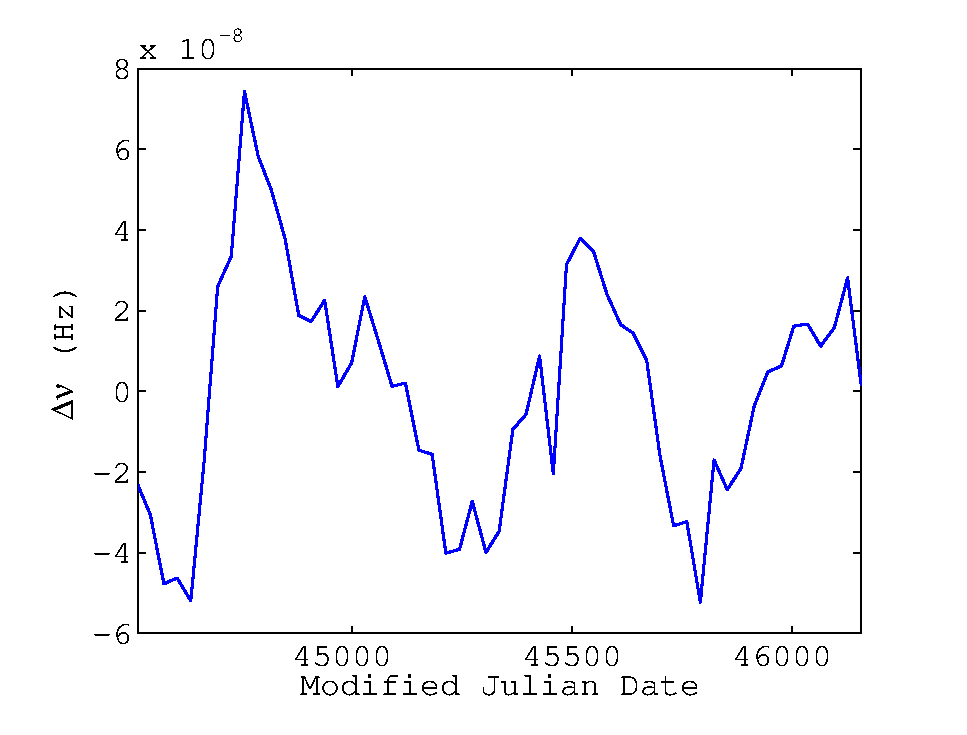
\includegraphics[width=0.6\textwidth]{figs/CrabTimingNoise}
\caption[Crab pulsar frequency timing noise.]{The timing noise in the frequency of the Crab pulsar
after removing a quadratic fit to the frequency as given in the Jodrell Bank ephemeris. Fit
parameters are given in table~\ref{CrabTimingNoiseParams}.}\label{CrabTimingNoise}
\end{center}
\end{figure}
\begin{table}[!htbp]
\caption{\label{CrabTimingNoiseParams} Parameters of fit for Crab pulsar frequency.}
\begin{center}
\begin{tabular}{| c | l |}
\hline
\multicolumn{2}{| c |}{PSR\,J0534+2200} \\
\hline \hline
$\nu$ & 30.05922413656965\,Hz \\
$\dot{\nu}$ & $-3.809951556460455\ee{-10}$\,Hz/s \\
$\ddot{\nu}$ & $1.207087526259945\ee{-20}$\,Hz/$\rm{s}^2$ \\
Frequency epoch & MJD 45015 \\
\hline
\end{tabular}
\end{center}
\end{table}
Figure~\ref{CrabTimingNoise} compares well the that given in Lyne {\it et al.} (1993)
\cite{Lyne:1993}, although some difference can be expected due to the different lengths of data and
epochs used in the fitting. It can be seen that on scales of several months there is quite a large
variation in the timing residual (including a possible 20 month quasi-sinusoidal periodicity shown
in Lyne {\it et al.}, 1988 \cite{Lyne:1988}). It is shown in \cite{Lyne:1993} that on smaller time
scales the variation is far smoother. The question that needs asking is whether a single model fit
for the Crab pulsar is going to be good enough to track the phase without significant phase
wandering, or whether the timing noise will mean that such a simple model would be too inaccurate to
track the phase. In Jones (2004) \cite{Jones:2004} a decoherence timescale, $T_{\rm{decoherence}}$,
is constructed as the time over which the timing noise will cause the phase to deviate by 1 radian
from the second order Taylor expansion of phase. This makes use of the ``activity parameter'' and is
calculated for the Crab pulsar to be $\sim 2.6$\,years. Using the activity parameter as a measure of
$T_{\rm{decoherence}}$ can be imprecise as it is not a fixed quantity and will vary with the model
fit epoch and time-span. The activity parameter will also not account for any permanent changes to
spin-down caused by glitches. $T_{\rm{decoherence}}$ should therefore not be taken as a hard and
fast value to adhere to. Another estimate of the effects of timing noise can also be made using the
$\Delta_8$ parameter, although for the Crab pulsar its value as derived from equation~\ref{delta8}
is not altogether useful. This is because for the Crab pulsar, unlike most other pulsars, timing
noise is not the dominant component in $\ddot{\nu}$, but is more a feature of even higher order
terms (although for the Crab pulsar even an intrinsic non-timing noise dominated value of
$\dddot{\nu}$ can be measured to an accuracy of 10\% \cite{PulsarAstronomy}). In Arzoumanian {\it et
al.} (1994) \cite{Arzoumanian:1994} they fit a linear relation between $\Delta_8$ and
$\log{\dot{P}}$ as
\begin{equation}\label{delta8slope}
\Delta_8 = 6.6 + 0.6\log{\dot{P}},
\end{equation}
where $\dot{P} = -\dot{\nu}/\nu^2$ is the period derivative, which we can use for the Crab pulsar
instead. This gives $\Delta_8 \approx -0.8$ which relates to a timing noise cumulative time offset
of $\sim 0.15$\,s or a phase offset of $\sim 4.4$\,cycles over a period of approximately three
years. A larger value than $T_{\rm{decoherence}}$ suggests.

It is reasonable that if a third order model for the Crab pulsar phase was fit over a period of a
few months, then it should fairly accurately represent the phase in that set of data. It is when the
stretch of data you need to cover extends for longer than this that such a fit breaks down. However
the Crab pulsar ephemeris provides timing every month, which should be sufficient to update the
model. By using the phase, frequency and frequency derivative for each entry in the ephemeris as
boundary conditions to a set of simultaneous equations the full phase evolution between each month
can be calculated, giving a fifth order equation,
\begin{eqnarray}\label{5thOrderPhase}
\phi_{5^{\rm th}}(t_b) & = & \phi_0 + 2\pi\Bigg\{\nu_0(t_b-t_0) + \frac{1}{2}\dot{\nu_0}(t_b-t_0)^2
\nonumber \\ 
& & + \frac{1}{6}\ddot{\nu_0}(t_b-t_0)^3 + \frac{1}{24}\dddot{\nu_0}(t_b-t_0)^4 +
\frac{1}{120}\ddddot{\nu_0}(t_b-t_0)^5\Bigg\}.
\end{eqnarray}
For most of the time this method might well be unnecessarily complicated and a simple linear
interpolation between months would be sufficient.

In terms of how this affects the analysis in \S\ref{TimeDomainMethod} it can be made equivalent to
performing an extra heterodyne step as described in Pitkin and Woan (2004) \cite{PitkinWoan:2004}.
In the initial heterodyne a third order fit to the the phase is used, with values of $\nu$ and
$\dot{\nu}$ taken from the ephemeris at the closest time \emph{before} the time of the data to be
analysed, and $\ddot{\nu}$ taken from the ATNF pulsar catalogue \cite{ATNF}. Then, assuming for the
moment that any \gw signal would also show timing noise, we apply a second heterodyne using the
phase difference between equations~\ref{PhaseTaylorExp} and \ref{5thOrderPhase}
\begin{equation}\label{extraheterodyne}
B_{k}' = B_ke^{-i2[\phi_{5^{\rm th}}(t_b) - \phi(t_b)]}.
\end{equation} 
This step can be performed on the $B_k$s after the filtering and down sampling as the rate of change
of this phase difference will be very slow.

The effect of this extra heterodyne can be seen using the example of the S2 analysis. This science
run of the LIGO interferometers lasted approximately two months and overlapped three entries in the
Crab pulsar ephemeris. The S2 run started on $14^{\rm{th}}$ Feb 2003, so values of the frequency and
spin-down used in the initial heterodyning were chosen to be those given in the first ephemeris
entry prior to the run (15th Jan 2003). The second derivative was set to be that taken from the ATNF
catalogue. The values shown in table~\ref{CrabS2Params} were multiplied by two to give the \gw
frequency.
\begin{table}[!htbp]
\caption{\label{CrabS2Params} The parameters used in the initial heterodyne stage of
the Crab pulsar analysis for S2.}
\begin{center}
\begin{tabular}{| c | l |}
\hline
\multicolumn{2}{| c |}{PSR\,J0534+2200} \\
\hline \hline
$\nu$ & 29.8102713888\,Hz \\
$\dot{\nu}$ & $-3.736982\ee{-10}$\,Hz/s \\
$\ddot{\nu}$ & $1.2426\ee{-20}$\,Hz/$\rm{s}^2$ \\
Frequency epoch & GPS\,726624013 \\
\hline
\end{tabular}
\end{center}
\end{table}
Once the $B_k$s were produced the ephemeris values were used to calculate the phase given in
equation~\ref{5thOrderPhase}. The difference between the initial heterodyne phase and the $5^{\rm
th}$ order phase is shown in figure~\ref{S2TimingNoisePhaseDiff}. 
\begin{figure}[!htbp]
\begin{center}
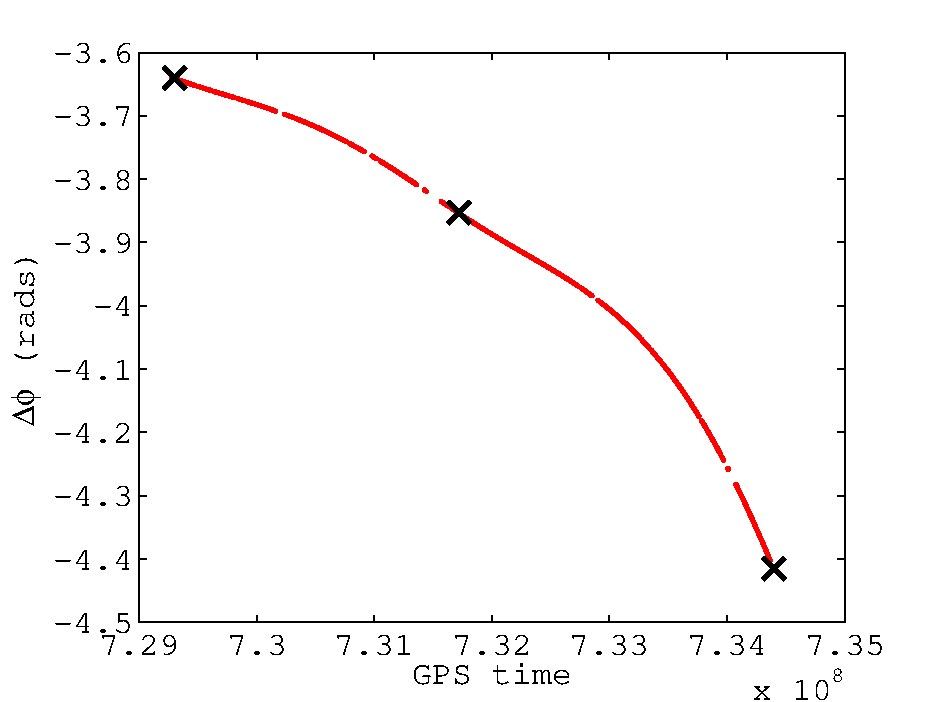
\includegraphics[width=0.6\textwidth]{figs/S2TimingNoisePhase}
\caption[Crab timing noise phase check during S2.]{The red points show the phase difference between
that used in the initial heterodyne and that interpolated from a fifth order fit to the ephemeris.
The black crosses show just the phase difference between the initial heterodyne and the individual
ephemeris values.}\label{S2TimingNoisePhaseDiff}
\end{center}
\end{figure}
This phase difference is used in the extra heterodyne to remove the variation. It can be seen in
figure~\ref{S2TimingNoisePhaseDiff} how a linear fit between ephemeris values would be acceptable
for these times, with only small deviations in phase from the fifth order fit. The black crosses in
figure~\ref{S2TimingNoisePhaseDiff} provide the first step in checking the code used for the extra
heterodyne stage. The red points represent the phase difference used in our extra heterodyne step
(equation~\ref{extraheterodyne}) to heterodyne each S2 data point as calculated using our code,
whereas the black crosses just show the phase difference between the initial heterodyne and the
individual Crab pulsar ephemeris data points. The fact that these overlap provides a check that the
heterodyne code is producing the correct phase difference. A second step in checking the code is to
make sure it introduces no spurious phase or amplitude changes to the $B_k$s. We can check the ratio
of the magnitudes of the $B_k$s before and after the timing noise heterodyne, $|B_{k~{\rm
before}}|/|B_{k~{\rm after}}|$. This ratio is equal to 1, bar tiny numerical noise, showing that
there are no unexpected amplitude changes introduced. We can also check that we can recover the
phase correction, $\Delta\phi(t) = 2[\phi_{5^{\rm th}}(t_b) - \phi(t_b)]$, using the $B_k$s before
($a = B_k$) and after ($b = B_ke^{-i\Delta\phi}$) the timing noise heterodyne is applied and the
relation
\begin{equation}
\frac{a\cdot{}b^{\ast}}{a\cdot{}a^{\ast}} =
\frac{B_k\cdot{}B_k^{\ast}e^{i\Delta\phi}}{B_k\cdot{}B_k^{\ast}} = e^{i\Delta\phi}.
\end{equation}
Using the identity $e^{i\Delta\phi} = \cos{\Delta\phi} + i\sin{\Delta\phi}$ the original phase
correction can be extracted. This extracted phase is shown in
figure~\ref{S2TimingNoisePhaseDiffCheck} and can be seen to be identical to that calculated and
shown in figure~\ref{S2TimingNoisePhaseDiff}.
\begin{figure}[!htbp]
\begin{center}
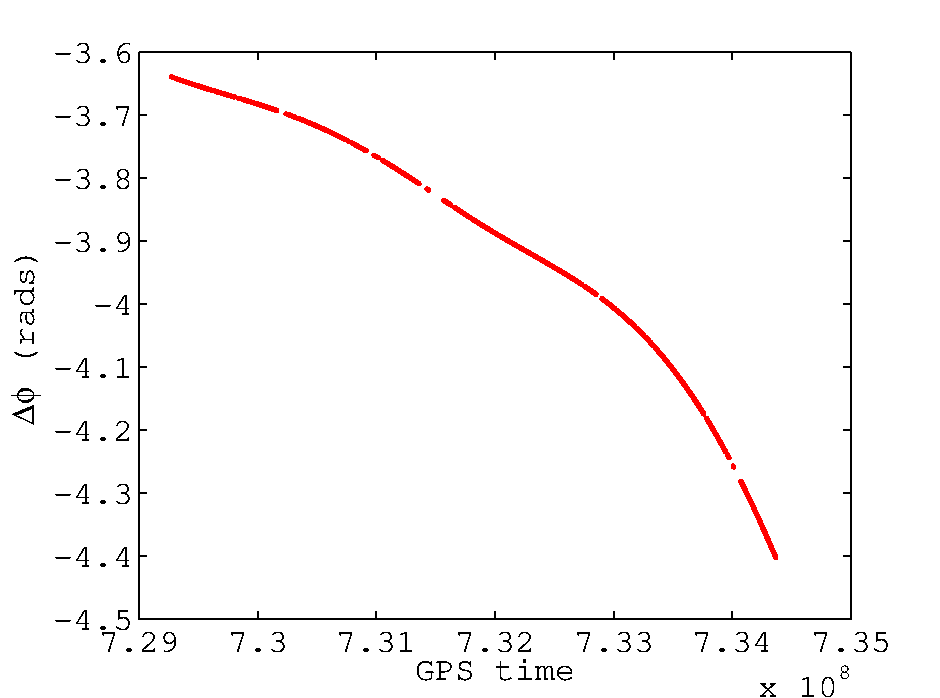
\includegraphics[width=0.6\textwidth]{figs/S2TimingNoisePhaseDiffCheck}
\caption{The timing noise phase correction as extracted from the $B_k$s before and
after heterodyning.}\label{S2TimingNoisePhaseDiffCheck}
\end{center}
\end{figure}

If we simulate a signal from the Crab pulsar over the period of S2 with the following parameters,
$h_0 = 0.5$, $\phi_0 = 0.0$, $\psi = 0.0$ and $\iota=\pi$, we can see how including a timing
noise heterodyne step affects the parameter estimation. Figure~\ref{S2CrabInjection} shows the
extracted values of $h_0$ and $\phi_0$ for the signal with and without the timing noise removed. It
can be seen that there is very little difference between the amplitudes for the two cases, due to
the slope of the phase difference $\Delta\phi$ not being too steep over the period of S2. 
\begin{figure}[!htbp]
\begin{center}
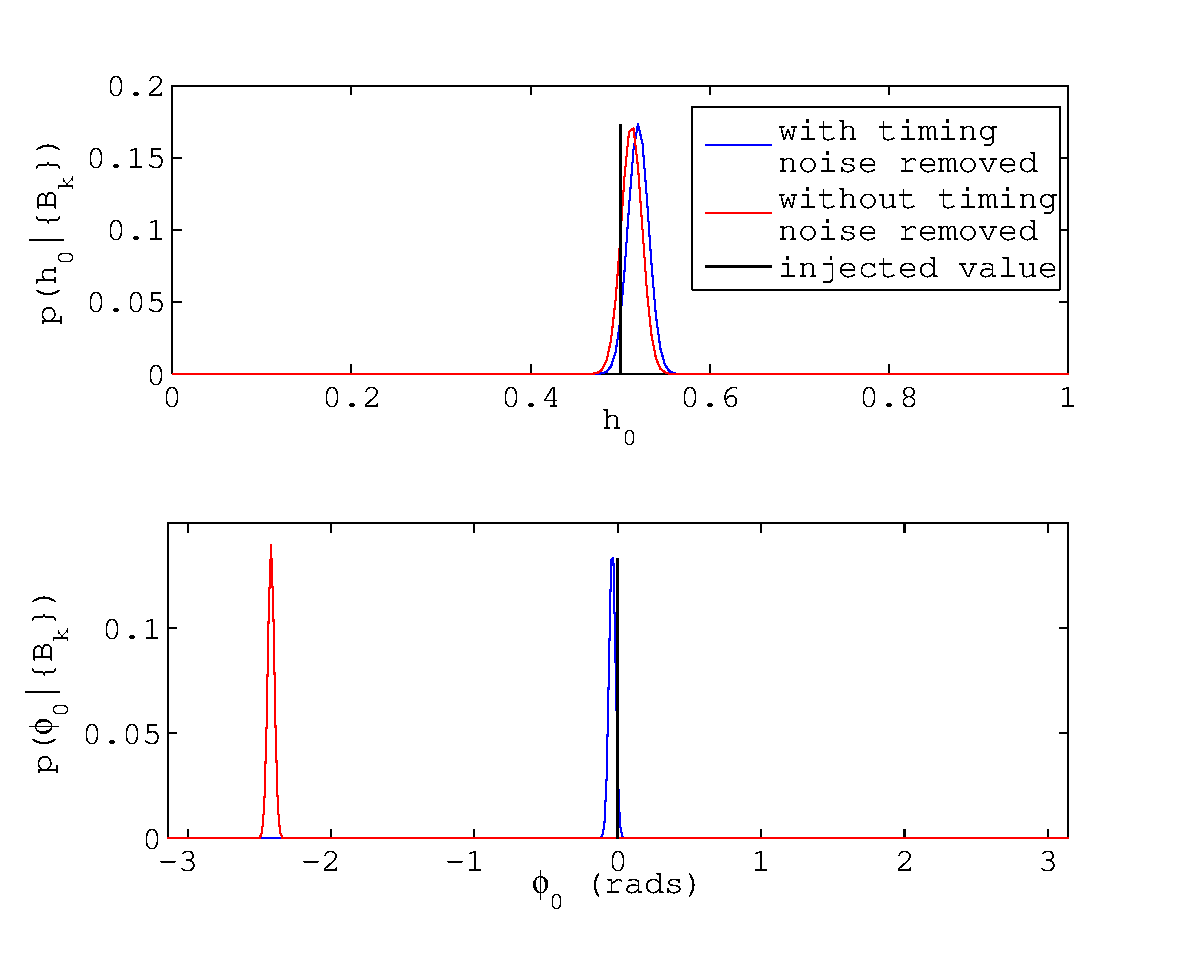
\includegraphics[width=0.5\textwidth]{figs/S2CrabInjection}
\caption{The extracted pdfs for $h_0$ and $\phi_0$ for a simulated signal from the
Crab pulsar over the period of S2 with and without timing noise removed.}\label{S2CrabInjection}
\end{center}
\end{figure}
However, the extracted value of the phase is affected quite heavily, mainly due to the the phase
offset between the start of S2 and the epoch of the initial heterodyne parameters seen in
figure~\ref{S2TimingNoisePhaseDiff}.

We can simulate a Crab pulsar signal and analyse it with and without the timing noise heterodyne
step over greater periods than just S2 to show its importance. The same process as above has been
carried out over the period of the S3 run, using the same initial heterodyne parameters and pulsar
injection parameters. The extracted pdfs can be seen in figure~\ref{S3CrabInjection} and show that
without the timing noise correction the signal is completely missed.
\begin{figure}[!htbp]
\begin{center}
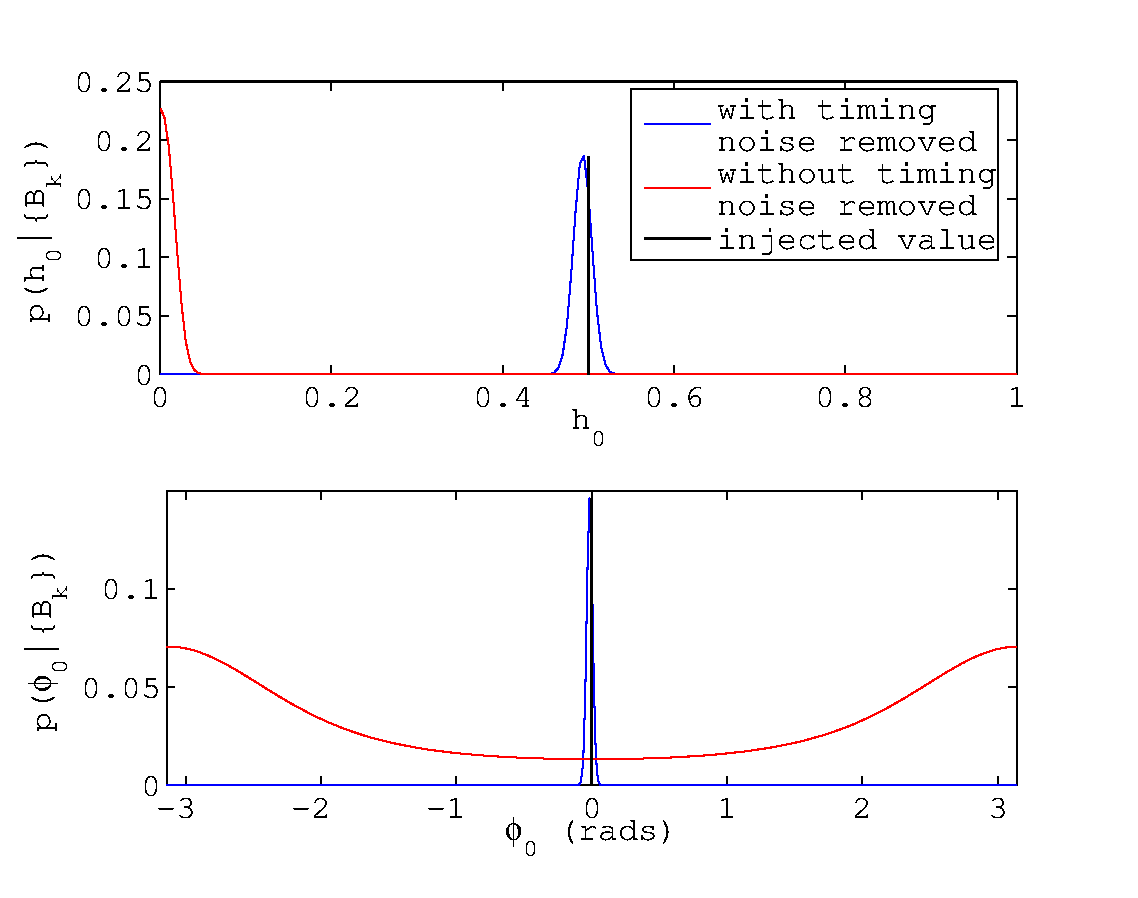
\includegraphics[width=0.5\textwidth]{figs/S3CrabInjection}
\caption{The extracted pdfs for $h_0$ and $\phi_0$ for a simulated signal from the
Crab pulsar over the period of S3 with and without timing noise removed.}\label{S3CrabInjection}
\end{center}
\end{figure}
The fact that the signal is not seen at all if the timing noise heterodyne is not used might seem
at odds with the 2.6 year decoherence time stated above, as S3 was only about 8 months after S2.
It is not seen however, because the initial heterodyne values used were chosen to be those from the
Crab ephemeris closest to the start of S2 and not those from a more general fit to the data over an
extended period, as was used to calculate $T_{\rm{decoherence}}$. If we perform a fit to the Crab
pulsar ephemeris over the whole of 2003, when the S2 and S3 took place, we can again check what
difference removing or not removing the timing noise has for S3 (see figure~\ref{S3CrabInjection2}).
\begin{figure}[!htbp]
\begin{center}
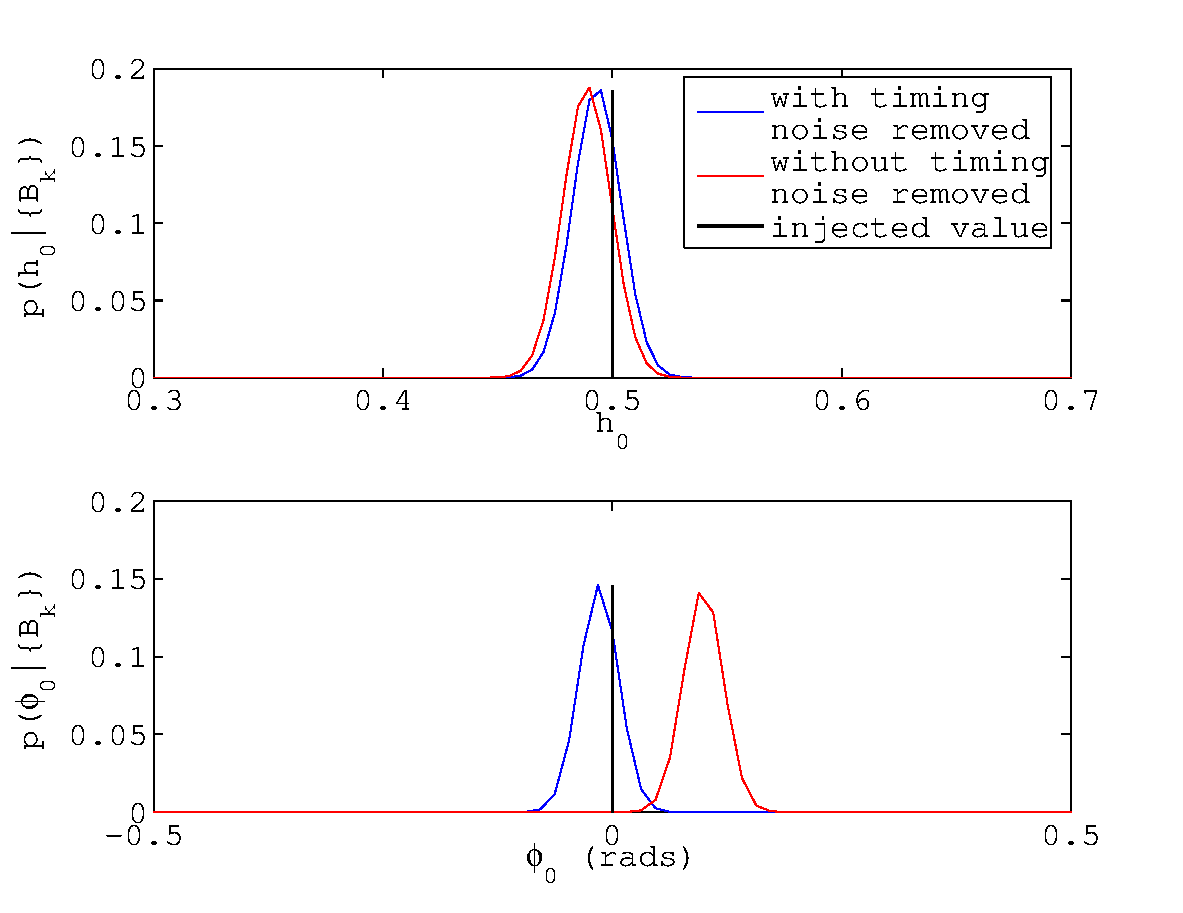
\includegraphics[width=0.5\textwidth]{figs/S3CrabInjection2}
\caption[Extracted pdfs of simulated Crab signal during S3.]{The extracted pdfs for $h_0$ and
$\phi_0$ for a simulated signal from the Crab pulsar over the period of S3 with and without timing
noise removed for initial heterodyne values obtained from a fit to the ephemeris over 2003 (see
table~\ref{CrabParams2003}).}\label{S3CrabInjection2}
\end{center}
\end{figure}
\begin{table}[!htbp]
\caption{\label{CrabParams2003} The parameters of the Crab for a fit to second order
in frequency over the period of 2003 using monthly ephemeris data.}
\begin{center}
\begin{tabular}{| c | l |}
\hline
\multicolumn{2}{| c |}{PSR\,J0534+2200} \\
\hline \hline
$\nu$ & 29.81027139567395\,Hz \\
$\dot{\nu}$ & $-3.736984315709851\ee{-10}$\,Hz/s \\
$\ddot{\nu}$ & $1.070857000427481\ee{-20}$\,Hz/$\rm{s}^2$ \\
Frequency epoch & GPS\,726624013.0597030 \\
\hline
\end{tabular}
\end{center}
\end{table}
Now it can be seen that for an extended fit for the Crab parameters whether or not the timing noise
is removed makes little difference over S3, although a slight phase offset is present. One might
then ask if it is then necessary to perform the extra timing noise heterodyne if fits to the pulsar
parameters over periods of say a year are good enough to provide the initial heterodyne parameters.
This is when the value of $T_{\rm{decoherence}}$ does come into play. For times scales less than
this a single heterodyne with properly fit parameters might be sufficient, although for long
observation times, as are required for continuous wave sources to build up $S/N$, it is best to
track the phase as accurately as possible. This also allows the maximum information to be extracted
if a detection occurs, as the electromagnetic and \gw phases can be compared accurately. Glitches in
the pulsar could also throw out the accuracy of any general fit, that a continuous updating of
parameters, as is done with the timing noise heterodyne stage, would not be sensitive to.

\subsection{Timing noise in other pulsars}
For the majority of pulsars timing noise is most prominent in the second derivative of frequency,
but for millisecond pulsars this value is often so small as to be unmeasurable. For these pulsars an
estimate of the effect of timing noise in terms of the $\Delta_8$ parameter can be made. This value
can be used to estimate the cumulative phase contribution of timing noise. As values of $\ddot{\nu}$
are so often unavailable values of $\Delta_8$ can be estimated via equation~\ref{delta8slope}. In
Chapter~3 this test will be used to examine the validity of the timing solutions for the selection
of pulsar in our analysis.

% fourth section will introduce the effects of pulsars in binary systems
\section{Pulsars in binary systems}\label{Binaries}
Of the 1533 pulsars in the ATNF catalogue some 112 are in binary systems. The first of which,
PSR\,J1915+1606, was discovered by Hulse and Taylor in 1974 \cite{HulseTaylor:1975}. Of these 112
pulsars 88 of them have spin frequencies greater than 25\,Hz (out of a total 150 isolated and binary
pulsars). The majority of millisecond pulsars are in binary systems. This disproportionally large
number of fast spinning pulsars in binary systems is unsurprising, as their rotation speed can be
attributed to the very fact that they have a companion. In such systems accretion of material from a
companion onto the pulsar results in it being spun-up as angular momentum is conserved. This process
is seen in LMXBs, where material accreting onto the neutron star is intensely heated and emits
X-rays. The Eddington limit suggests that there must be a limit on the rate of accretion where it
matches the rate at which the star can lose energy. Assuming the energy is lost through magnetic
dipole radiation a limit on the pulsar period from accretion spin-up can be given by
\begin{equation}
P = 1.9B_9^{6/7} \rm{milliseconds},
\end{equation}
where $B_9$ is the magnetic field strength on the stars surface in units of $10^9$\,gauss
\cite{PulsarAstronomy}. It its shown in figure~10.1 of Lyne and Graham-Smith (1998)
\cite{PulsarAstronomy} that the majority of millisecond pulsars fall below this limit. Of course
this is assuming accretion energy is only lost via dipole radiation and discounting the possibility
of energy loss via \gw emission. A limit on the spin period of recycled\footnote{pulsars spun-up by
accretion.} millisecond pulsars supposing \gw emission plays a role in energy loss is given in
Andersson (1999) \cite{Andersson:1999}. The mechanism for producing this limit will only be in play
during the accreting stage when the neutron star is hot. It is believed that all millisecond pulsars
are recycled and belonged to binary systems for which, in the case of now isolated pulsars, a
subsequent disruption, i.e. a supernova explosion or merger, caused the loss/expulsion of the
companion star. Millisecond pulsars have a magnetic field several orders of magnitude lower than the
slower population meaning that their spin-down rate (due to magnetic dipole radiation) is
significantly lower and they will continue to spin at high speeds over a long period.

\subsection{Pulsar timing}
A brief discussion on how pulsar timing information is obtained is relevant here. The majority of
pulsars have been discovered and are monitored using radio telescopes. Searches, discussed in
more detail in Lyne and Graham-Smith (1998) \cite{PulsarAstronomy}, in general use Fourier transform
methods to look for periodic signals in the radio telescope output. Radio astronomers also take
into account, and fit, the effect of interstellar dispersion across the radio frequency band which
they observe, whereby electrons in the interstellar medium slow down electromagnetic waves as
a function of frequency. This dispersion measure will depend on the density of the ISM through which
the radio waves have had to travel. Once a pulsar signal is detected timing measurements can be
made. Over short periods of time the time series radio data can be folded at the pulsar frequency to
build up the $S/N$ of the actual pulse. Once a stable pulse is obtained\footnote{individual pulses
can vary in shape, but the summation of many gives a generally stable pulse shape.} the time
of arrival (TOA) can be measured at the peak of the pulse. 
% chunk removed and shifted to the TEMPO comparison section
These pulse times can then be used to extract more precise information about the pulsar parameters,
including its position and frequency parameters. 

The most prevalent tool used by pulsar astronomers for fitting timing measurements is the \tempo
software \cite{TEMPO}. This requires precise solar system ephemerides, containing the positions and
velocities of the major solar system bodies, to convert TOAs at a detector to the rest frame of
the pulsar. It computes the pulsar phase at each TOA, $\phi(T_i)$, over the range of pulsar
parameters ($\alpha$, $\delta$, $\nu$, $\dot{\nu}$, etc), and uses a $\chi^2$ goodness of fit
statistic to determine the best model via minimisation. A starting point for the fit is obtained
through a rough knowledge of the position and frequency from the initial discovery, but it can still
be quite complex as there can be many other parameters that could be contributing. Below it is seen
how a pulsar in a binary system requires a complex model with many more parameters than an isolated
object.

\subsection{Binary pulsar timing}
The fact that the majority of pulsars within our \gw frequency band are in binary systems means
that in any search for known pulsars, if we want to maximise the number of potential sources, then
we need to look into how this will effect the search described above. This has not been used or
described before in previous pulsar \gw searches. Equation~\ref{TimeDelay} shows the timing
corrections needed to take account of Doppler and relativistic delays to a signal and transform
it to the SSB. As is generally the case any additional Doppler delays from the pulsar's actual
motion relative to the SSB are negligible and the SSB frame can be considered as the rest frame of
the pulsar. For a pulsar in a binary system this will not be the case and its motion within the
system will need to be taken into account. To achieve this a transform from binary
system barycentre to the pulsar proper time is needed.

The basic transformation and binary models below are summarised in Taylor and Weisberg (1989)
\cite{TaylorWeisberg:1989} and used in the pulsar timing program \tempo \cite{TEMPO}. The
transformation from SSB time $t_b$ (in TT) to pulsar proper time $T$ follows the form of 
equation~\ref{TimeDelay} and is
\begin{equation}\label{SSBtoPPT}
t_b - t_0 = T + \Delta_{\rm{R}} + \Delta_{\rm{E}} + \Delta_{\rm{S}} + \Delta_{\rm{A}},
\end{equation}
where $\Delta_{\rm{R}}$ is the Roemer time delay giving the propagation time across the binary
orbit; $\Delta_{\rm{E}}$ is the Einstein delay and gives gravitational redshift and time dilation
corrections; $\Delta_{\rm{S}}$ is the Shapiro delay and gives general relativistic correction; and
$\Delta_{\rm{A}}$ is the aberration delay caused by the pulsars rotation. When radio astronomers
search for pulsars in binary systems they need to have a model of that system to calculate the
transformation to proper time. For the majority of systems the orbits can be described as Keplerian
(just governed by Newtonian gravity and following Kepler's laws). Such Keplerian orbits are defined
by five parameters, $T_0$ - the time of periastron (closest approach in the binary orbit); $\omega$
- the longitude of periastron; $P_b$ - the orbital period; $e$ - the orbital eccentricity (where $e
= \sqrt{(1-b^2/a^2)}$ and $a$ and $b$ are the semi-major and semi-minor axis of the orbital ellipse
respectively); and $x \equiv (a\sin{i})/c$ is the projected semi-major axis, with $i$ being the
orbital inclination. We will look at the three main models used by radio pulsar astronomers to
describe binary systems.

\subsubsection{Blandford-Teukolsky model}
The first model put forward for use in describing pulsars in binary systems was that of Blandford
and Teukolsky \cite{BlandfordTeukolsky:1976} (BT), which provided a model that made no assumptions
about the correct relativistic theory of gravity. This model assumes a Keplerian orbit with slow
precession, into which additional relativistic effects have been added. Other phenomena can be taken
into account through time derivatives of the four main orbital elements excluding $T_0$. As shown in
\cite{TaylorWeisberg:1989} equation~\ref{SSBtoPPT} becomes
\begin{eqnarray}\label{BT}
\lefteqn{t_b - t_0 = T + \{x\sin{\omega}(\cos{E} - e) + [x\cos{\omega}(1-e^2)^{1/2} +
\gamma]\sin{E}\}} \nonumber \\
& & \times \Big\{1 - \frac{2\pi}{P_b}[x\cos{\omega}(1 - e^2)^{1/2} \cos{E} - x\sin{\omega}\sin{E}]
\nonumber \\
& & \times (1 - e\cos{E})^{-1}\Big\},
\end{eqnarray}
where $\gamma$ incorporates gravitational redshift and time dilation effects, and $E$ is the
eccentric anomaly as defined via Kepler's equation,
\begin{equation}\label{KeplersEquation}
E - e\sin{}E = \frac{2\pi}{P_b}(t_b - T_0).
\end{equation}
The eccentric anomaly can be well approximated by power series in $e$ as in Dhurandhar and Vecchio
(2001) \cite{DhurandharVecchio:2001}, but in practice it is often easier to solve iteratively. Any
additional relativistic effect can be fit via the inclusion of $\dot{\omega}$, $\dot{P_b}$,
$\dot{x}$ and $\dot{e}$, so for example $\omega = \omega_0 + \dot{\omega}(t_b - T_0)$. The BT model
has been used to fit data for 47 of the binary pulsars with $\nu > 25$\,Hz, so is the most common
model used. One of these systems is modelled using the \tempo model BT2P which accommodates three
orbits, the first of which can be relativistic, but the second and third are Keplerian. The system
is a multiple system, described in Wolszczan {\it et al.} (2000) \cite{Wolszczan:2000}, in which
three, or possibly four, planets orbit the pulsar. Although additional orbits complicate the above
equations it has been suggested to us by Michael Kramer \cite{Kramer:2004} that the ordinary BT
model is good enough to describe the system for our purposes.

\subsubsection{Low eccentricity model}
The second most common model used in fitting radio observations of binaries is the low eccentricity
model (called ELL1 in T\textsc{empo}) developed in Lange {\it et al.} (2001) \cite{Lange:2001}. It
is used as a fit for pulsars in very low eccentricity orbits where $e$ is almost zero and is the
model for 34 of the pulsars with $\nu > 25$\,Hz. With an almost circular orbit it is very hard to
fit a value of $T_0$ and $\omega$, so these parameters, along with $e$, are replaced with the time
of the ascending node of the orbit ($T_{\rm{asc}} \equiv T_0 - \omega{}P_b/2\pi$) and the first and
second Laplace-Lagrange parameters $\eta \equiv e\sin{\omega}$ and $\kappa \equiv e\cos{\omega}$.
The time delays for this model, defined in \cite{Lange:2001} and the \tempo code, are
\begin{eqnarray}\label{ELL1DRE}
\Delta_{\rm{R}} + \Delta_{\rm{E}} = & \Delta_{\rm{RE}} =&  x\left(\sin{\Phi} +
\frac{\kappa}{2}\sin{2\Phi} - \frac{\eta}{2}\cos{2\Phi}\right),\\
& \Delta_{\rm{RE}}\prime = & x\cos{\Phi}, \\
& \Delta_{\rm{RE}}\prime\prime = & -x\sin{\Phi}, \\
& \Delta_{\rm{S}} = & -2r{\rm{ln}}(1 - s \sin{\Phi}), \\
& \Delta_{\rm{A}} = & A_0\sin{\Phi} + B_0\cos{\Phi},
\end{eqnarray}
where the phase of the orbit is $\Phi = \frac{2\pi}{P_b}(t_b-T_{\rm{asc}})$, $r=Gm_2/c^3$ is the
Shapiro range parameter for a companion mass $m_2$, $s = \sin{}i$ is the Shapiro shape parameter,
and $A_0$ and $B_0$ are abberation coefficients. Time derivatives for the parameters are taken
into account with the reference epoch now being $T_{\rm{asc}}$. The time delay thus becomes
\begin{equation}\label{ELL1DT}
t_b - t_0 = T + \Delta_{\rm{RE}}\left(1 - \frac{2\pi}{P_b}\Delta_{\rm{RE}}\prime +
\frac{4\pi^2}{P_b^2}\Delta_{\rm{RE}}\prime^2 +
\frac{2\pi^2}{P_b^2}\Delta_{\rm{RE}}\Delta_{\rm{RE}}\prime\prime\right) + \Delta_{\rm{S}} +
\Delta_{\rm{A}}.
\end{equation}
The inclusion of the Sharpiro shape and range parameters means that, under strong-field gravity 
conditions, this model can provide more information about the nature of the system than the BT
model. These parameters are nearly degenerate and can show up as a small correction to the observed
ellipticity. For the majority of systems the effect of the $\Delta_{\rm{S}}$ term is negligible. The
abberation delay coefficients will also be small and are also degenerate with other values, so the
$\Delta_{\rm{A}}$ term will contribute very little. In \tempo the abberation coefficients are not
included in the model fitting procedure although they can be set to a fixed value if desired.

\subsubsection{Damour-Deruelle model}
The third most common model is the Damour-Deruelle (DD) model \cite{DamourDeruelle:1986}. This
model uses a method for solving the relativistic two-body problem to post-Newtonian order and is
valid under very general assumptions about the nature of gravity in strong field regimes. It is
useful for highly relativistic systems where the most information needs to be extracted from the
timing solution. There are six pulsars with $\nu >25$\,Hz in the ATNF catalogue using this model.
This model is again summarised in \cite{TaylorWeisberg:1989} with the various time delays given by
\begin{eqnarray}\label{DDdelays}
\Delta_{\rm{R}} & = & x\sin{\omega} [\cos{E} - e(1 + \delta_r)] \nonumber \\ 
 & & + x[1 - e^2(1 + \delta_{\theta})^2]^{1/2} \cos{\omega} \sin{E}, \\
\Delta_{\rm{E}} & = & \gamma\sin{E}, \\
\Delta_{\rm{S}} & = & -2r\log{}\{1 - e\cos{E} - s [\sin{\omega} (\cos{E} - e) \nonumber \\
 & & + (1-e^2)^{1/2} \cos{E} \sin{E}]\}, \\
\Delta_{\rm{A}} & = & A_0\{\sin{[\omega + A_e(E)]} + e\sin{\omega}\} \nonumber \\
& & + B_0\{\cos{[\omega + A_e(E)]} + e\cos{\omega}\},
\end{eqnarray}
where the eccentric anomaly is now defined via Kepler's equation as
\begin{equation}
E -  e\sin{E} = 2\pi\left[\left(\frac{T-T_0}{P_b}\right) -
\frac{\dot{P_b}}{2}\left(\frac{T-T_0}{P_b}\right)^2\right],
\end{equation}
and the true anomaly $A_e(E)$ is given by
\begin{equation}
A_e(E) = 2\arctan{\left[\left(\frac{1+e}{1-e}\right)^{1/2}\tan{\frac{E}{2}}\right]}.
\end{equation}
The time derivative of $\omega$ now comes into the equation via $\omega = \omega_0 + kA_e(E)$, where
$k = \dot{\omega}P_b/2\pi$, but the other time derivatives and $\gamma$ are essentially the same as
for the BT model. The abberation coefficients and parameters $\delta_r$ and $\delta_{\theta}$ are
again small and nearly degenerate with other parameters, making the $\Delta_{\rm{A}}$ term
negligible.

\subsection{Comparison with TEMPO}
The above three models are all implemented in the pulsar timing software package T\textsc{empo}. In
our search for \gws from binary systems we also require these additional time corrections to
correctly calculate the phase of the pulsar for heterodyning. Code to calculate the binary time
delays for each model have been adapted from their \tempo counterparts and are available under CVS
in the LALapps repository \cite{LALapps}. Some consistency tests have been performed between the two
codes, which are described below.

\subsubsection{PSR\,J1012+5307}
A convincing check of the LALapps code is to use it to demodulate a signal from a radio pulsar. To
do this Michael Kramer supplied us with a set of TOAs for PSR\,J1012+5307 obtained with the
Effelsberg 100\,m radio telescope in Bonn, Germany. This pulsar has the second most circular
orbit known and hence requires the ELL1 model. The data spanned just over 5 years\footnote{from
$2^{\rm{nd}}$ January 2000 to $12^{\rm{th}}$ February 2005} of on and off observations of the
pulsar, and was supplied in the form of TOAs in MJD\footnote{Modified Julian Date = Julian Date -
2400000.5} with timing errors in $\mu{}s$ and the observing frequency. We were also supplied with
the \tempo fit to the pulsar parameters (see table~\ref{PSRJ1012+5307}).
\begin{table}[!htbp]
\caption[The parameters of PSR J1012+5307.]{\label{PSRJ1012+5307} The parameters of PSR J1012+5307.
Values are quoted with $1\sigma$ errors in brackets.}
\begin{center}
\begin{tabular}{| l | l |}
\hline
\multicolumn{2}{| c |}{PSR\,J1012+5307} \\
\hline \hline
$\alpha$ & $10^{\rm{h}}12^{\rm{m}}33^{\rm{s}}.43368(1)$ \\
$\delta$ & $53^{\circ}07'02''.5880(2)$ \\
PMRA   & 2.38(3)\,mas/yr \\
PMDEC  & $-25.35$(5)\,mas/yr \\
$\nu$  & 190.267837621884(9)\,Hz \\
$\dot{\nu}$ & $-6.2022(2)\ee{-16}$\,Hz/s \\
$\ddot{\nu}$ & $2.0(3)\ee{-27}$\,Hz/$\rm{s}^2$ \\
Frequency epoch & MJD\,50700 \\
Dispersion measure & 9.0233(7)\,${\rm{cm}}^{-3}$\,pc \\
Observing Frequency  & 1408.6\,MHz \\
Binary model & ELL1 \\    
$x$ & 0.581817(1)\,s \\
$P_b$ & 0.6046727136(2)\,days \\
$T_{\rm{asc}}$ & MJD\,50700.0816289(4) \\
$\eta$  &  $7(4)\ee{-7}$ \\
$\kappa$  &  $-1(40)\ee{-8}$ \\
\hline
\end{tabular}
\end{center}
\end{table}

There were several correction that needed to be made to the supplied TOAs to convert them from the
time system measured at the radio telescope to GPS. The first correction to the raw TOAs was to
correct for the difference between the stable Hydrogen maser time source at the telescope and
coordinate Universal Time of the National Institute of Science and Technology UTC(NIST) reference,
supplied by Michael Kramer. This correction was typically of order a few $\mu$s. The next
correction that could have been made was the conversion from UTC(NIST) to UTC although this has been
less than $\pm 100$\,ns since $6^{\rm{th}}$ July,
1994\footnote{\url{http://tf.nist.gov/timefreq/pubs/bulletin/nistutc2000.htm}} so in practice was
left out. The conversion between time in UTC times (given in MJD) to GPS times then follows as
$t_{\rm{GPS}} = (t_{\rm{UTC(MJD)}} - 44244\,{\rm{days}})\times86400\,{\rm{s}} + {\rm{leap
seconds}}$, where the 44244\,days is the MJD of the GPS time epoch ($1^{\rm{st}}$ January, 1980)
and the leap seconds represent the difference between UTC and GPS required as UTC is adjusted to
match the Earth's rotation. For the times span of our given TOAs the number of leap seconds was
always 13.

The next step was to correct the times for interstellar dispersion. The dispersion time
delay is given by
\begin{equation}
\Delta{}t_{\rm{disp}} =
4.148808\ee{3}\,{\rm{MHz}}^2\,{\rm{pc}}^{-1}\,{\rm{cm}}^3\,{\rm s}\times{\rm{DM}}/f^2\,{\rm s},
\end{equation}
where DM is the dispersion measure in ${\rm{cm}}^{-3}$\,pc and $f$ is the radio observation
frequency in MHz (see table~\ref{PSRJ1012+5307} for values). This correction is subtracted from the
TOAs to give observations at infinite frequency with no dispersion. 

The next stage compared the publicly available LIGO Algorithm Library (LAL) \cite{LAL}
barycentring codes to T\textsc{empo}. As the pulsar parameters were calculated using \tempo we can
check whether our barycentring codes can use these values to match the pulsar's phase. One of the
major differences between our binary time domain code and the \tempo code is the time system used.
All epochs in \tempo are defined in Barycentric Dynamical Time (TDB) whereas the general reference
time for \gw data analysis in the LSC is GPS time. Epochs can be converted to Barycentric
Dynamical Time (TDB), which is a generally used timescale for ephemerides referenced to the solar
solar barycentre. This timescale is related to Terrestrial Time (TT - formerly Terrestrial Dynamical
Time TDT), which represents a time consistent with relativity for an observer on the Earth's
surface, by a small factor, $\rm{TDB} = \rm{TT} + \delta{}t$, no greater than a couple of
milliseconds and given by
\begin{equation}
\delta{}t = 0.001\,658\,{\rm s}\times\sin{\Phi} + 0.000\,014\,{\rm s}\times\sin{2\Phi},
\end{equation}
where $\Phi = 357.53^{\circ} + 0.985\,600\,28^{\circ}(\rm{MJD} - 51\,544.5)$ is the mean anomaly, or
phase, of the Earth's orbit at the given Modified Julian Date. TT is related to International
Atomic Time (TAI) via TT = TAI + 32.184 seconds\footnote{There are many definitions of time used in
astronomy and very careful attention of which one is being used and how to convert between them is
essential when high precision timings are being made. A good guide to these is given at
\cite{Times}.} The conversion from TT to GPS time, therefore meant subtracting 51.184\,s, where
32.184\,s comes from the difference between TT and TAI and the remaining 19\,s are the number of
leap seconds between TAI and GPS. The code to calculate the SSB time delay takes in the pulsar's
position, the telescope position and a solar system ephemeris\footnote{the ephemerides used are
those published by the Jet Propulsion Laboratory \cite{JPLEphemeris}.} and was used for each pulsar
TOA to correct to the time at the SSB. This code was written by Curt Culter and has been
independently tested against \tempo \cite{Abbott:2004, Dupuis:2004} showing no more than $4\,\mu$s
difference between the two. Once corrected to the SSB the TOAs then needed to be corrected to the
pulsar proper time by calculating the time delays in the binary system using the binary system
parameters (see table~\ref{PSRJ1012+5307}). The binary and solar system time delays for a selection
of TOAs covering part of the binary orbit are shown in figure~\ref{J1012+5307DT}.
\begin{figure}[!htbp]
\begin{center}
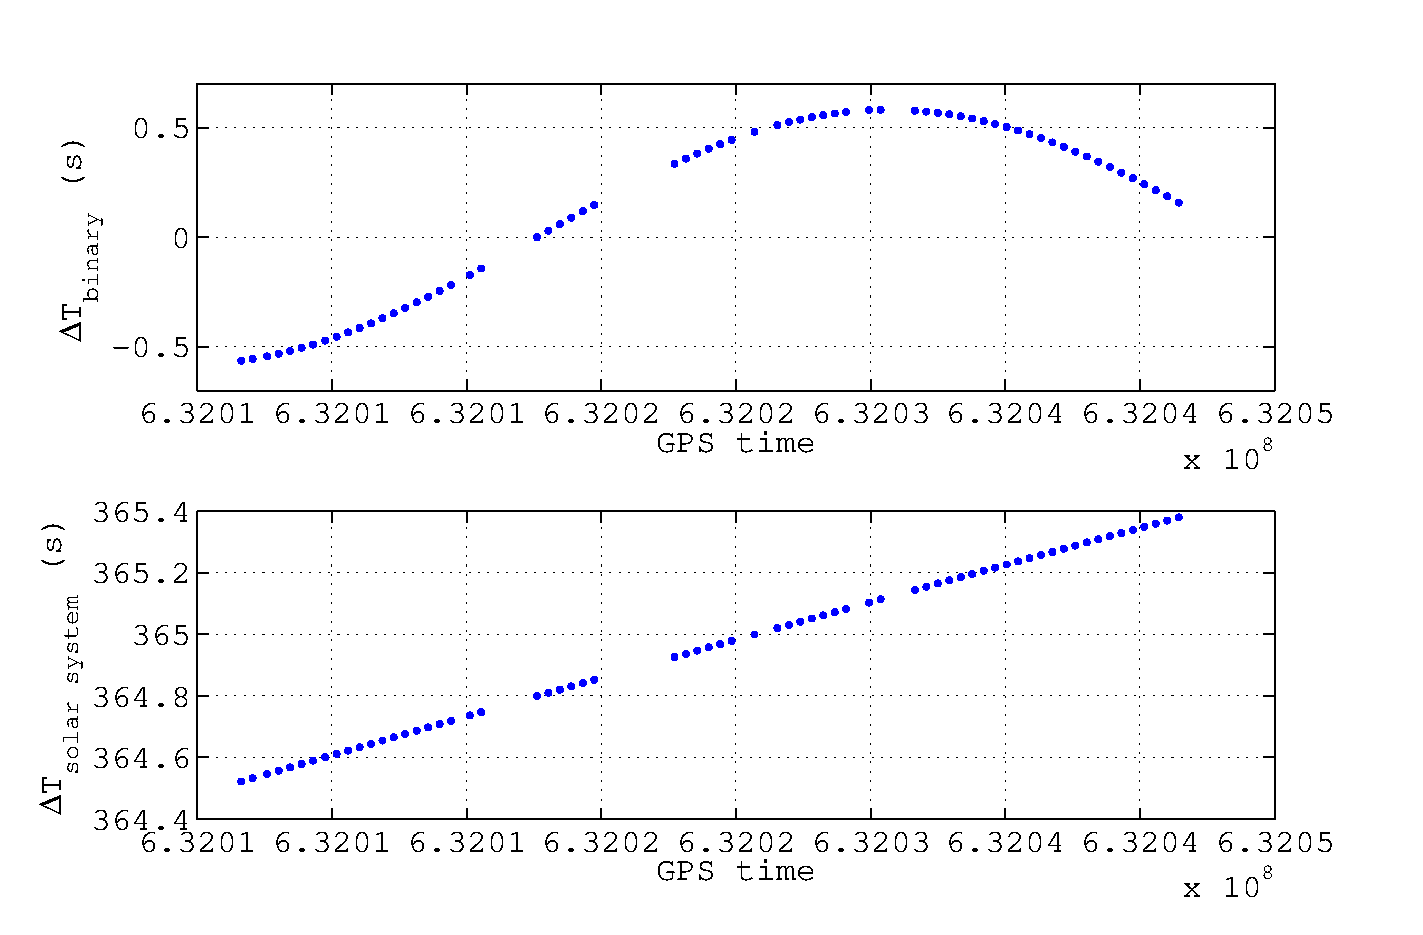
\includegraphics[width=0.6\textwidth]{figs/J1012+5307DT}
\caption[The binary and solar system time delays for PSR\,J1012+5307.]{The binary and solar system
time delays calculated for PSR\,J1012+5307 over a part of an orbit.}\label{J1012+5307DT}
\end{center}
\end{figure}
Once the corrections to the TOA had been applied the phase could be checked. All TOAs should be in
phase as they each represent the peak of a pulse. If the TOAs were incorrectly converted by the
barycentring codes then this would show up by them being out of phase. The phase at each TOA was
calculated using the supplied frequency and frequency derivatives in equation~\ref{PhaseTaylorExp},
with $\phi_0 = 0$ and the frequency epoch as $t_0$.
\begin{figure}[!htbp]
\begin{center}
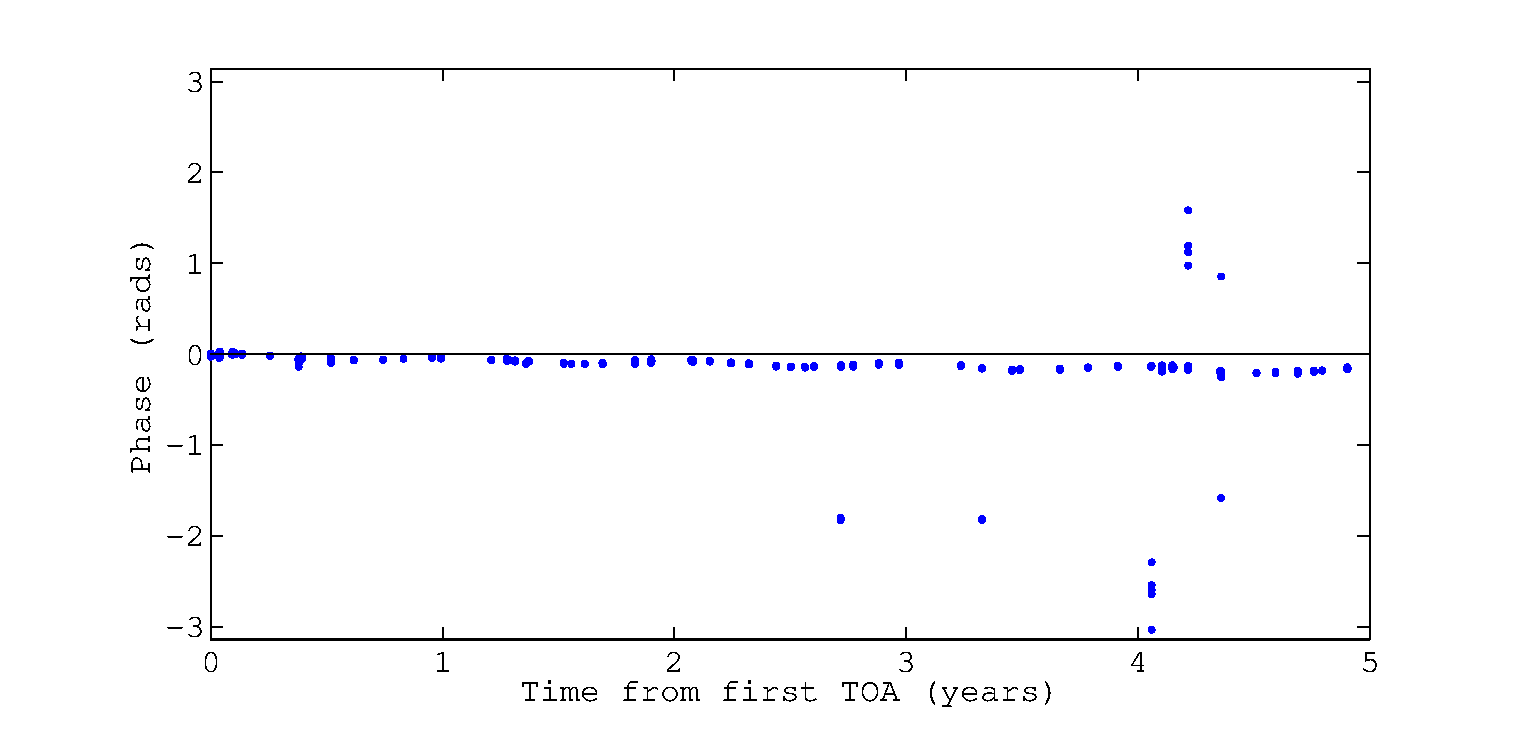
\includegraphics[width=0.6\textwidth]{figs/J1012+5307Phase}
\caption{The modulus of the pulsar phase at each TOA over a 5 year period.}\label{J1012+5307Phase}
\end{center}
\end{figure}
Figure~\ref{J1012+5307Phase} shows how the TOAs barycentred using our code stay in phase well over
the observation time. There is a slight slope of $\sim 0.04$\,rads/yr in the phase. A yearly
periodicity is also present possibly showing up the slight difference in the LAL solar
system barycentring code and T\textsc{empo}, although these effects are at a very low level. There
are several points that are quite out of phase which correspond to times when the level of noise on
the TOA measurements was high.

The parameters for PSR\,J1012+5307 were generated using the ELL1 model, so the above test really
only checked the code describing that model. We can also check the two other models by converting
$T_{\rm{asc}}$ to $T_0$ and the Laplace-Lagrange parameters $\kappa$ and $\eta$ to $e =
\sqrt{(\kappa^2+\eta^2)}$ and $\omega$. As this pulsar has such a low eccentricity then $T_0$ can be
set equal to $T_{\rm{asc}}$ and $\omega$ set to zero. Doing this we can again produce the phase
plots for the BT and DD models (figure~\ref{J1012+5307BT_DDPhase}).
\begin{figure}[!htbp]
\begin{center}
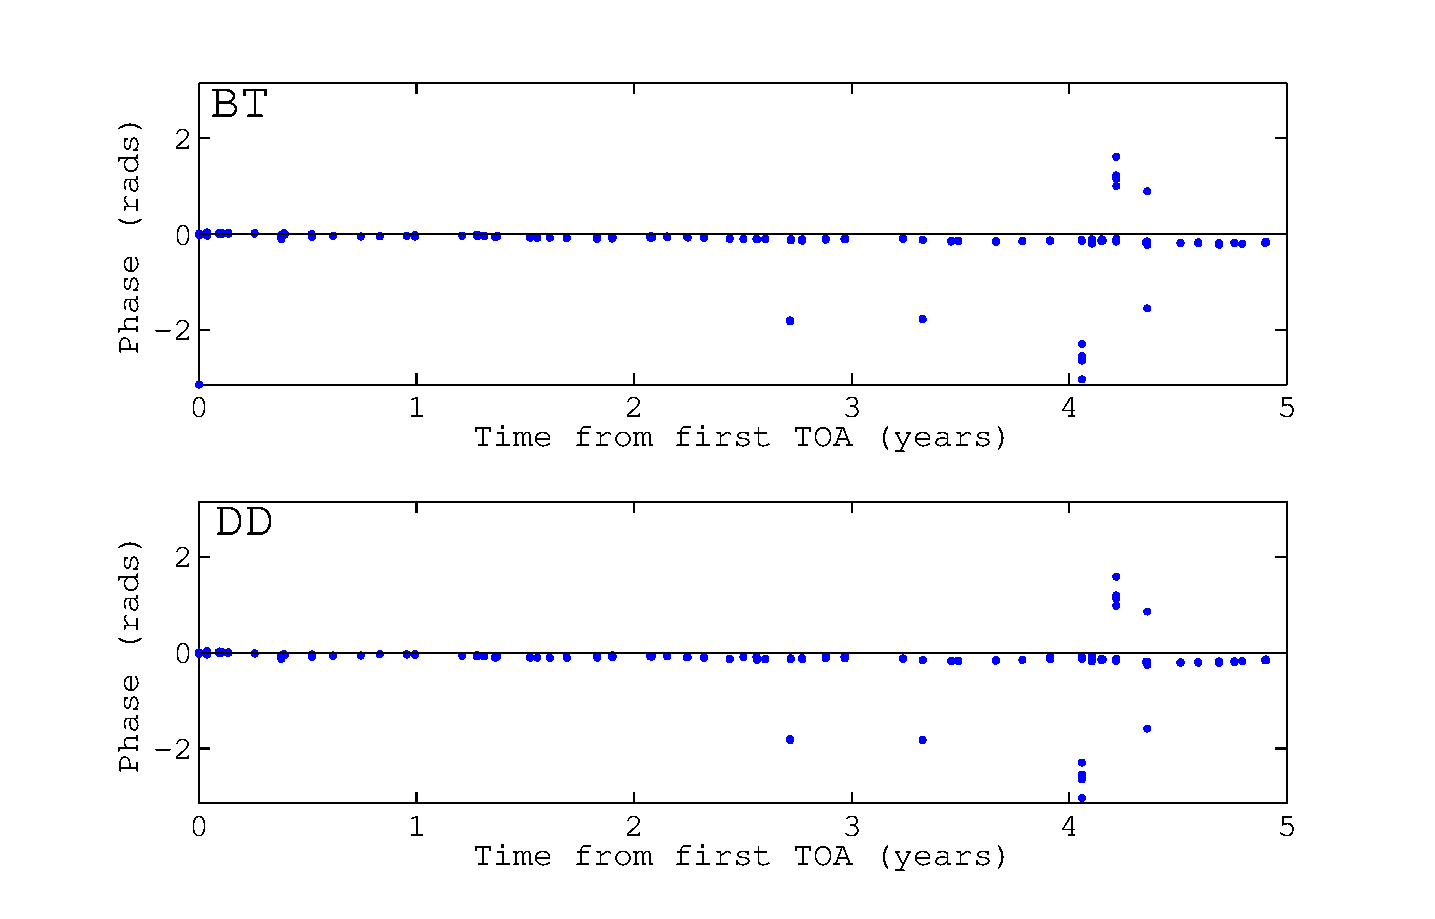
\includegraphics[width=0.6\textwidth]{figs/J1012+5307BT_DDPhase}
\caption{The modulus of the pulsar phase at each TOA over a 5 year period for the BT
and DD models.}\label{J1012+5307BT_DDPhase}
\end{center}
\end{figure}
The phase is again well described for these two models, with the slope and periodicity still
present. This suggests that the slope and periodicities are not caused by the binary timing
correction code (as each model is independent), but may be a results of slight errors in the other
timing corrections, the solar system barycentring code or the parameters used.

\subsubsection{Direct check against TEMPO}
As was done for the solar system barycentring code, the binary timing code can be tested directly
against T\textsc{empo}. \tempo can be set into the so called predictive mode, whereby it uses a set
of pulsar parameters to predict the pulsar phase over a period of time. This predicted phase can be
then be compared with that calculated using our binary timing code. This was done for each model
with a set of 500 randomly generated binary pulsar systems over a period of 100 days. The
detector location was set to be at the SSB, so the solar system time delay errors would not be
included. Histograms of the time residuals between the codes are shown in
figure~\ref{TEMPOComparison} for each model.
\begin{figure}[!htbp]
\begin{center}
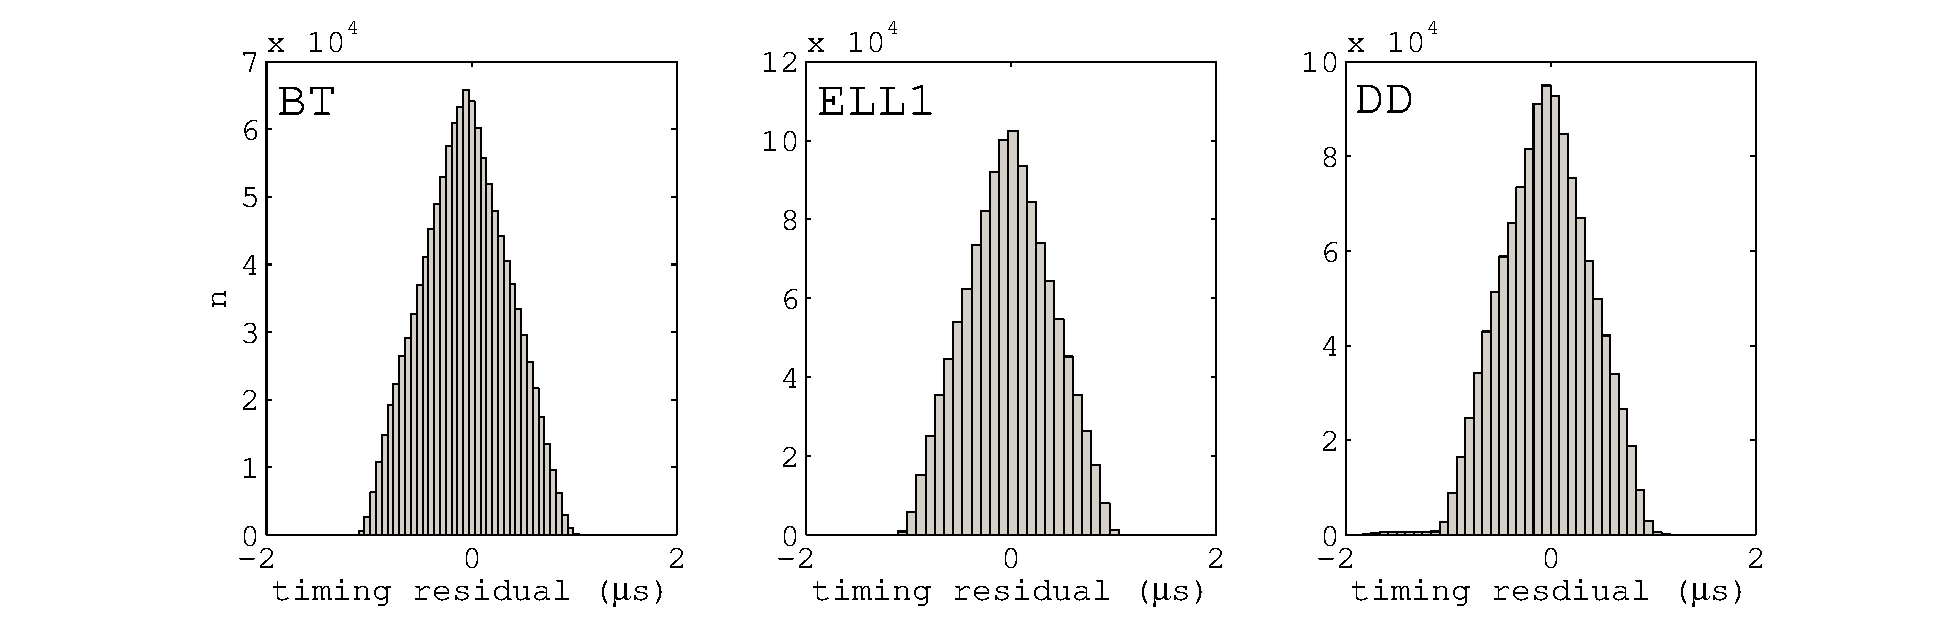
\includegraphics[width=1.0\textwidth]{figs/TEMPOComparison}
\caption[Timing residuals between our code and T\textsc{empo}.]{Timing residuals between the pulsar
phase as predicted by \tempo and that computed with our binary code for 500 random pulsars for each
binary model.}\label{TEMPOComparison}
\end{center}
\end{figure}
These show that the time difference between the two codes is generally less than $\pm1\,\mu$s,
meaning there is a very good agreement between the codes and sufficient accuracy to ensure any
signal and template remain in phase.